\documentclass{llncs}

\usepackage{makeidx}

\usepackage{bm}
\usepackage{pgfplots}
\usepackage{enumerate,paralist}
\usepackage{pbox}
\usepackage{parskip}
\usepackage{multirow}
\usepackage{url}

%\usepackage{subfigure}
%\usepackage{appendix}
%\usepackage{comment}

\usepackage{graphicx}
\usepackage{tikz,pgffor}
\usetikzlibrary{arrows}
\usetikzlibrary{shapes}
\usetikzlibrary{calc}
\usetikzlibrary{automata}
\usetikzlibrary{positioning}

\tikzstyle{location}=[rectangle, rounded corners, draw=black, very thick, minimum height=2em, inner sep=0pt,text centered]
\tikzstyle{tran}=[draw,->,>=stealth, rounded corners]
\tikzstyle{dec}=[inner sep=0pt]
\tikzstyle{mode}=[shape=circle,draw,inner sep=0pt,minimum size=5mm]

\usepackage{lmodern}
\usepackage{amsmath}
\usepackage{amssymb}
%\usepackage{amsthm}

\usepackage{mathtools}
\usepackage{times}
\usepackage{stmaryrd}

%\theoremstyle{plain}
%\newtheorem{lemma}{Lemma}
%\newtheorem{claim}{Claim}
%\newtheorem{proposition}{Proposition}
%\newtheorem{definition}{Definition}
%\newtheorem{corollary}{Corollary}
%\newtheorem{theorem}{Theorem}
%\newtheorem{example}{Example}
%\newtheorem{remark}{Remark}
%\newtheorem{observation}{Observation}
%\newtheorem{assumption}{Assumption}

%% Notations

%%General Notations

\newcommand{\Rset}{\mathbb{R}}
\newcommand{\Nset}{\mathbb{N}}
\newcommand{\Zset}{\mathbb{Z}}
\newcommand{\ap}{\mbox{\sl AP}}
\newcommand{\opt}{\mbox{\sl opt}}

%%Clocks and Clock Constraints

\newcommand{\clocks}{\mathcal{X}}
\newcommand{\val}[1]{\mbox{\sl Val}\left(#1\right)}
\newcommand{\reset}[2]{{#1}{\left[#2:=0\right]}}
\newcommand{\add}[2]{{#1}{+}{#2}}
\newcommand{\zero}{\mathbf{0}}
\newcommand{\true}{\mathbf{true}}
\newcommand{\false}{\mathbf{false}}
\newcommand{\supp}[1]{{\mbox{\sl supp}}(#1)}
\newcommand{\dist}[1]{{\mathcal{D}}{\left(#1\right)}}
\newcommand{\sat}[1]{{\llbracket}{#1}{\rrbracket}}
\newcommand{\intp}[1]{{\lfloor}{#1}{\rfloor}}
\newcommand{\fracp}[1]{\mbox{\sl frac}(#1)}
\newcommand{\evclass}[1]{\left[#1\right]}

%%PTAs

\newcommand{\pta}{\mathcal{C}}
\newcommand{\locs}{L}
\newcommand{\loc}{\ell}
\newcommand{\acts}{\mbox{\sl Act}}
\newcommand{\inv}{\mbox{\sl inv}}
\newcommand{\enab}{\mbox{\sl enab}}
\newcommand{\prob}{\mbox{\sl prob}}
\newcommand{\lbfunc}{\mathcal{L}}
\newcommand{\clcons}[1]{\mbox{\sl CC}\left(#1\right)}
\newcommand{\istate}{\left(\loc^*,\mathbf{0}\right)}

%% Semantics of PTAs

\newcommand{\states}{S}
\newcommand{\trans}{\rightarrow}
\newcommand{\tran}[3]{{#1}{\xrightarrow{#2}}{#3}}
\newcommand{\probk}{\mathbf{P}}
\newcommand{\fnpaths}[1]{\mbox{\sl Paths}^*_{#1}}
\newcommand{\infpaths}[1]{\mbox{\sl Paths}^\omega_{#1}}
\newcommand{\omgpaths}[2]{\mbox{\sl Reach}^{#2}_{#1}}
\newcommand{\initloc}[1]{\mbox{\sl init}\left(#1\right)}

\newcommand{\fnpath}{\rho}
\newcommand{\infpath}{\pi}

%% Notations for Probability Space

\newcommand{\probm}{\mathbb{P}}
\newcommand{\expv}{\mathbb{E}}
\newcommand{\cyl}{\mbox{\sl Cyl}}

%% Notations for DTAs

\newcommand{\dta}{\mathcal{A}}
\newcommand{\dtloc}{q}
\newcommand{\cstates}{Q}
\newcommand{\alphabet}{\Sigma}
\newcommand{\fstates}{F}
\newcommand{\rules}{\Delta}
\newcommand{\dtphi}[3]{\Phi_{#1,#2}^{#3}}
\newcommand{\dtx}[3]{\mathbf{X}_{#1,#2}^{#3}}
\newcommand{\dtq}[3]{\mathbf{q}_{#1,#2}^{#3}}
\newcommand{\trfunc}{\kappa}
\newcommand{\dtatr}[3]{{#1}{\xRightarrow{#2}}{#3}}
\newcommand{\regions}{\mathcal{G}}

\newcommand{\run}[3]{{#1}_{#2}\left(#3\right)}
\newcommand{\iconfig}{\left(\dtloc^*,\mathbf{0}\right)}

%%Product Constrution
\newcommand{\product}[2]{{#1}{\otimes}{#2}}
\newcommand{\pr}[2]{\mathfrak{p}_{#1}^{#2}}
\newcommand{\pfunc}{\mathcal{T}}
\newcommand{\sfunc}{\theta}
\newcommand{\acc}[2]{{\mbox{\sl AccPaths}}_{#1}^{#2}}
\newcommand{\extactions}{\mathcal{B}}
\newcommand{\exttuples}{\mathcal{T}}

%%Reward Structure
\newcommand{\rcum}{\mathbf{r}_{\locs}}
\newcommand{\rinst}{\mathbf{r}_{\acts}}
\newcommand{\ronestep}{\mathbf{r}}
\newcommand{\accum}[1]{\mbox{\sl Cum}_{#1}}
\newcommand{\rd}[2]{\mathsf{R}_{#1}^{#2}}

%%Rabin acceptance

% \newcommand{\infset}[1]{\mbox{\sl{inf  }} ( #1 )}
% \newcommand{\trace }[1]{\mbox{\sl{trace}} ( #1 )}
% \newcommand{\traj  }[1]{\mbox{\sl{traj }} ( #1 )}
\newcommand{\infset}[1]{inf  ( #1 )}
\newcommand{\trace }[1]{trace( #1 )}
\newcommand{\traj  }[1]{traj ( #1 )}
\newcommand{\rabin}{\mathcal{F}}

\newcommand{\Lang}[2] {
    Lang
        _{#1}
        ^{#2}
}

\newcommand{\Accept}[2]{
    Accept
        _{#1}
        ^{#2}   
}

\newcommand{\LangCsAqF}{
    \Lang
        {\pta,\sigma}
        {\dta,\dtloc,\rabin}
}

\newcommand{\AcceptCxAqsF}{
    \Accept
        {
            \product{\pta}{\dta_\dtloc},
            \sigma
        }
        {\rabin}
}

\newcommand{\TLang}{
    \pfunc\left(
        \LangCsAqF
    \right)
}

\newcommand{\TAcc}{
    \Accept
        {
            \product{\pta}{\dta_\dtloc},
            \sfunc \left( 
                \sigma
            \right)
        }
        {\rabin}
}


%%For drawing grids

\newcounter{row}
\newcounter{col}

\newcommand\setrow[3]{
  \setcounter{col}{1}
  \foreach \n in {#1, #2, #3} {
    \edef\x{\value{col} - 0.5}
    \edef\y{3.5 - \value{row}}
    \node[anchor=center] at (\x, \y) {\n};
    \stepcounter{col}
  }
  \stepcounter{row}
}

% Undecidability
\newcommand{\nta}{\mathcal{A}}
\newcommand{\qinit}{q_{init}}
\newcommand{\ntaap}[1]{p_{#1}}
\newcommand{\PCswLang}{
    \probm^{\pta,\sigma_w }\left(
    \Lang
        {\pta,\sigma_w}
        {\nta',\qinit,\rabin}
    \right)
}
%%adjusting layout

%\renewcommand{\baselinestretch}{0.96}
%\addtolength{\textheight}{0.1in}
%\addtolength{\voffset}{-0.05in}
%\addtolength{\oddsidemargin}{-0.05in}
%\addtolength{\evensidemargin}{-0.05in}
%\addtolength{\textwidth}{0.1in}
\addtolength{\parskip}{-0.5mm}
%\setlength{\textfloatsep}{0.2cm}

\begin{document}

\title{Verifying Probabilistic Timed Automata Against \\Deterministic-Timed-Automata Specifications}
\titlerunning{Verifying PTAs against DTA specifications}

\author{Hongfei Fu\inst{1}, Yi Li\inst{2}, Jianlin Li\inst{3}, Lijun Zhang\inst{1}}
\authorrunning{Hongfei Fu et al.}

\institute{State Key Laboratory of Computer Science\\ Institute of Software, Chinese Academy of Sciences, Beijing, China
\and
Department of Informatics, School of Mathematical Sciences\\ Peking University, Beijing, China,
\and
College of Computer Science and Technology \\Nanjing University of Aeronautics and Astronautics, Nanjing, China}
%Formal Methods and Tools Group, The University of Twente, The Netherlands}
%College of computer science and technology, Nanjing University of Aeronautics and Astronautics, Nanjing, P.R. China
\maketitle

\begin{abstract}
Probabilistic timed automata (PTAs) are timed automata extended with discrete probability distributions.
They serve as a mathematical model for a wide range of applications that involve both stochastic and timed behaviours.
In this paper, we study the model-checking problem of linear \emph{dense-time} temporal properties over PTAs.
In particular, we consider linear dense-time properties that can be encoded by timed automata with both finite and infinite acceptance criteria.
We first show that the problem of model-checking PTAs against deterministic-timed-automata specifications with infinite acceptance criterion can be solved through a product construction and is EXPTIME-complete.
Then we show that when relaxed to general (nondeterministic) timed automata, the model-checking problem becomes undecidable.
Finally, we investigate the situation where the acceptance criterion is restricted to be finite. 
We show that for deterministic timed automata, the model-checking problem can be solved
using known zone-based algorithms for reachability probabilities on PTAs.
Furthermore, for nondeterministic timed automata, we show an approximation algorithm for solving the problem whose correctness is based on a translation to infinite-state Markov decision processes.
\end{abstract}

% \vspace{-0.8em}
\section{Introduction}
% \vspace{-0.8em}
Stochastic timed systems are systems that exhibit both timed and stochastic behaviours.
Such systems play a dominant role in many real-world applications (cf.~\cite{DBLP:books/daglib/0020348}), hence
addressing fundamental issues such as safety and performance over these systems are important.
\emph{Probabilistic timed automata} (PTAs)~\cite{DBLP:journals/fmsd/NormanPS13,DBLP:journals/tcs/Beauquier03,DBLP:journals/tcs/KwiatkowskaNSS02} serve as a good mathematical model for these systems.
They extend the well-known model of timed automata~\cite{DBLP:journals/tcs/AlurD94} (for nonprobabilistic timed systems) with discrete probability distributions, and Markov Decision Processes (MDPs)~\cite{PutermanMDP} (for untimed probabilistic systems) with timing constraints.

Formal verification of PTAs has received much attention in recent years~\cite{DBLP:journals/fmsd/NormanPS13}.
For branching-time model checking of PTAs, the problem is reduced to computation of reachability probabilities over MDPs through well-known finite abstraction for timed automata (namely \emph{regions} and \emph{zones})~\cite{JensenPTA,DBLP:journals/tcs/Beauquier03,DBLP:journals/tcs/KwiatkowskaNSS02}.
Advanced techniques for branching-time model checking of PTAs such as inverse method and symbolic method have been explored in  ~\cite{DBLP:journals/fmsd/AndreFS13,DBLP:journals/iandc/KwiatkowskaNSW07,DBLP:conf/formats/KwiatkowskaNP09,DBLP:conf/formats/JovanovicKN15}.
Extension with \emph{cost} or \emph{reward}, resulting in \emph{priced} PTAs, has also been investigated.
On one hand, Berendsen \emph{et al.}~\cite{DBLP:conf/tamc/BerendsenCJ09} proved that cost-bounded reachability probability is undecidable over priced PTAs.
On the other hand, Jurdzinski~\emph{et al.}~\cite{DBLP:conf/concur/JurdzinskiKNT09} and Kwiatkowska~\emph{et al.}~\cite{DBLP:journals/fmsd/KwiatkowskaNPS06} proved that several notions of accumulated (discounted) cost are computable over priced PTAs.
Most verification algorithms for PTAs have been implemented in the model checker PRISM~\cite{DBLP:conf/cav/KwiatkowskaNP11}. Computational complexity of several verification problems for PTAs is studied in~\cite{DBLP:journals/ipl/LaroussinieS07,DBLP:journals/lmcs/JurdzinskiSL08,DBLP:conf/concur/JurdzinskiKNT09}.

A shortcoming of existing verification approaches for PTAs is that they all considered branching-time properties.
As far as we know, no results have ever considered linear-time model checking for PTAs.
Linear-time temporal properties are however important as they can specify complex timed behaviours induced by e.g. finite sequences of timed events.
In particular, we focus on linear-time temporal properties that can be encoded by deterministic timed automata (DTAs).
DTA is the deterministic version of timed automata.
Although DTA is weaker than general timed automata, it can recognize a wide class of formal timed languages, and express interesting properties which cannot be expressed in branching-time logics~\cite{DBLP:journals/tse/DonatelliHS09}.
The problem to verify DTA-specifications over stochastic timed models has only been investigated for continuous-time Markov processes (cf.~\cite{DBLP:journals/tse/DonatelliHS09,DBLP:journals/corr/abs-1101-3694,DBLP:conf/hybrid/Fu13,DBLP:conf/hybrid/BrazdilKKKR11,DBLP:conf/tacas/BarbotCHKM11,DBLP:conf/formats/BortolussiL15}), a completely different formalism for stochastic timed systems which assigns probability distributions to time elapses.
In this paper, we study verification of DTA-specifications over PTAs.
As far as we know, we are the first to conduct this line of research.

\textbf{Our Contributions.} We show that through a product construction, the optimal probability of PTA-paths accepted by a DTA w.r.t the finite acceptance criterion can be computed exactly by known algorithms for reachability probabilities over PTAs.
The novelty of our product construction is that to enable the DTA to keep track of the next location after a probabilistic jump in the PTA, one needs to integrate either the set of regions of the DTA or a local conjunction over the rules of the DTA.
%Then we show that migrating from finite acceptance criteria to Rabin criteria can be handled by maximal end components. Finally, we show that under almost-sure acceptance w.r.t finite acceptance condition, the expected accumulated cost/reward until acceptance can be computed through known algorithms for priced PTAs.
We demonstrate experimental results on several case studies and show that our approach is effective to analyse linear-time properties over PTAs.
%\textbf{Organization of the Paper.} Section~\ref{?} introduces some preliminaries. Section~\ref{?} describes the problem studied in this paper. Section~\ref{} is the core part of this paper which demonstrates the product construction.
%Section~\ref{?} illustrates several case studies.
%Finally, Section~\ref{?} show our experimental results and Section~\ref{?} concludes the paper.
\vspace{-0.8em}
\section{Preliminaries}
\vspace{-0.8em}

In the whole paper, we denote by $\Nset$, $\Nset_0$, $\Zset$, and $\Rset$ the sets of all positive
integers, non-negative integers, integers, and real numbers, respectively.

For an infinite string $w$, $\infset{w}$ is the set of symbols that occur infinitely many times in $w$.
\vspace{-0.8em}
\subsection{Clock Valuations, Clock Constraints and Clock Equivalences}
\vspace{-0.8em}

In this part, we fix a finite set $\clocks$ of \emph{clocks}.

\noindent{\em Clock Valuations.} Let $\clocks$ be a finite set of \emph{clocks}.
A \emph{clock valuation} is a function $\nu:\clocks\rightarrow [0,\infty)$. The set of clock valuations
is denoted by $\val{\clocks}$.
Given a clock valuation $\nu$, a subset $X\subseteq\clocks$ of clocks and a non-negative real number $t$, we let (i) $\reset{\nu}{X}$ be the clock valuation such that $\reset{\nu}{X}(x)=0$ for $x\in X$ and $\reset{\nu}{X}(x)=\nu(x)$ otherwise, and (ii) $\add{\nu}{t}$ be the clock valuation such that $(\add{\nu}{t})(x)=\nu(x)+t$ for all $x\in\clocks$.
Moreover, we denote by $\zero$ the clock valuation such that $\zero(x)=0$ for all $x\in\clocks$.

\noindent{\em Clock Constraints.} The set of \emph{clock constraints} $\clcons{\clocks}$ over $\clocks$ is generated by the following grammar:
\[
\phi:=~\true~\mid~x\le d~\mid ~c\le x~\mid~x+c\le y+d~\mid ~\neg\phi~\mid~\phi\wedge\phi
\]
where $x,y\in\clocks$ and $c,d\in\Nset_0$.
We write $\false$ for a short hand of $\neg\true$.
The satisfaction relation $\models$ between valuations $\nu$ and clock constraints $\phi$ is defined through substituting every $x\in\clocks$ appearing in $\phi$ by $\nu(x)$ and standard semantics for logical connectives.
For a given clock constraint $\phi$, we denote by $\sat{\phi}$ the set of all clock valuations that satisfy $\phi$.

\noindent{\em Clock Equivalence.} Consider a nonnegative integer $N$ which acts a threshold for relevant clock values: values held by clocks are treated the same if they exceed $N$.
With such a fixed $N$, the standard notion of clock equivalence (see~\cite{DBLP:journals/tcs/AlurD94}) is an equivalence relation $\sim_N$ over $\val{\clocks}$ as follows: for any two clock valuations $\nu,\nu'$, $\nu\sim_N\nu'$ iff the following conditions hold:
\begin{compactitem}
\item for all $x\in\clocks$, $\nu(x)>N$ iff $\nu'(x)> N$;
\item for all $x\in\clocks$, if $\nu(x)\le N$ then (i) $\intp{\nu(x)}=\intp{\nu'(x)}$ and (ii) $\fracp{\nu(x)}>0$ iff $\fracp{\nu'(x)}>0$;
\item for all $x,y\in\clocks$, if $\nu(x),\nu(y)\le N$ then $\fracp{\nu(x)}\Join \fracp{\nu(y)}$ iff $\fracp{\nu'(x)}\Join \fracp{\nu'(y)}$ for all $\Join\in\{<,=,>\}$.
\end{compactitem}
Equivalence classes of $\sim_N$ are conventionally called \emph{regions}. The equivalence class that contains a given clock valuation $\nu$ is conventionally denoted by $\evclass{\nu}_\sim$.
\vspace{-0.8em}
\subsection{Probabilistic Timed Automata}
\vspace{-0.8em}
To introduce the notion of probabilistic timed automata (PTAs), we first define the notion of discrete probability distributions.

\noindent{\em Discrete Probability Distributions.} A \emph{discrete probability distribution} over a countable non-empty set $U$ is a function $q:U\rightarrow[0,1]$ such that $\sum_{z\in U}q(z)=1$.
The \emph{support} of $q$ is defined as $\supp{q}:=\{z\in U\mid q(z)>0\}$.
The set of discrete probability distributions over $U$ is denoted by $\dist{U}$.
For $u \in U$, let $\mu(u)$ be the \emph{point distribution at $u$} which assigns probability 1 to $u$.

\vspace{-0.8em}
\begin{definition}[Probabilistic Timed Automata (PTAs)~\cite{DBLP:journals/fmsd/NormanPS13}]
A \emph{probabilistic timed automaton} (PTA) $\pta$ is a tuple
\begin{equation}\label{eq:pta}
\pta=\left(\locs, \loc^*, \clocks, \acts, \inv, \enab,  \prob, \lbfunc\right)
\end{equation}
where
\begin{compactitem}
\item $\locs$ is a finite set of \emph{locations} and $\loc^*\in\locs$ is the \emph{initial} location;
\item $\clocks$ is a finite set of \emph{clocks};
\item $\acts$ is a finite set of \emph{actions};
\item $\inv:\locs\rightarrow\clcons{\clocks}$ is
%a function which assigns to every location
an \emph{invariant condition};
\item $\enab:\locs\times\acts\rightarrow\clcons{\clocks}$ is an \emph{enabling condition};
\item $\prob:\locs\times\acts\rightarrow\dist{2^{\clocks}\times\locs}$ is a \emph{probabilistic transition function};
\item $\ap$ is a finite set of \emph{atomic propositions} and $\lbfunc:\locs\rightarrow 2^{\ap}$ is a \emph{labelling function}.
\end{compactitem}
\end{definition}
\vspace{-0.8em}

W.l.o.g, we assume that both $\acts$ and $\ap$ is disjoint from $[0,\infty)$. Below we fix a PTA $\pta$ in the form (\ref{eq:pta}). The semantics of PTAs is as follows.

\noindent{\em States and Transition Relation.}
A \emph{state} of $\pta$ is a pair $(\loc, \nu)$ in $\locs\times\val{\clocks}$ such that $\nu\models \inv(\loc)$.
The set of all states is denoted by $\states_\pta$.
The \emph{transition relation} $\trans$ consists of all triples $((\loc,\nu),a,(\loc',\nu'))$ satisfying that
\begin{compactitem}
\item $(\loc,\nu), (\loc',\nu')$ are states and $a\in\acts\cup [0,\infty)$;
\item if $a\in [0,\infty)$ then $\nu+\tau\models \inv(\loc)$ for all $\tau\in [0, a]$ and $(\loc',\nu')=(\loc,\nu+a)$;
\item if $a\in\acts$ then $\nu\models\enab(\loc,a)$ and there exists a pair $(X, \loc'')\in\supp{\prob(\loc,a)}$ such that $(\loc',\nu')=(\loc'',\reset{\nu}{X})$.
\end{compactitem}
By convention, we write $\tran{s}{a}{s'}$ instead of $(s,a,s')\in\trans$.
We omit the subscript `$\pta$' in `$\states_\pta$' if the underlying context is clear.
The \emph{probability transition kernel} $\probk$ is the function $\probk:\states\times\acts\times\states\rightarrow[0,1]$ such that
\[
\probk((\loc,\nu),a,(\loc',\nu'))=\begin{cases}
1 & \mbox{if }\tran{(\loc,\nu)}{a}{(\loc',\nu')}\mbox{ and } a\in [0,\infty)\\
\sum_{Y\in B}\prob(\loc,a)(Y,\loc') & \mbox{if }\tran{(\loc,\nu)}{a}{(\loc',\nu')}\mbox{ and } a\in\acts \\
0 & \mbox{otherwise}
\end{cases}
\]
where $B:=\{X\subseteq\clocks\mid \nu'=\reset{\nu}{X}\}$.

\noindent{\em Well-formedness.} We say that $\pta$ is \emph{well-formed} if for every state $(\loc,\nu)$ and action $a\in\acts$ such that $\nu\models\enab(\loc,a)$ and for every $(X,\loc')\in \supp{\prob(\loc,a)}$, one has that $\reset{\nu}{X}\models\inv(\loc')$.
The well-formedness is to ensure that when an action is enabled, the next state after taking this action will always be legal. In the rest of the paper, we always assume that the underlying PTA is well-formed. PTAs that are not well-formed can be repaired to satisfy the well-formedness condition~\cite{DBLP:journals/iandc/KwiatkowskaNSW07}.

\noindent{\em Paths.}
A \emph{finite path} $\fnpath$ (under $\pta$) is a finite sequence
\[
\left\langle s_0,a_0,s_1,\dots,a_{n-1},s_n\right\rangle~~(n\ge 0)
\]
in $\states\times{\left((\acts\cup[0,\infty))\times \states\right)}^*$
such that (i) $s_0=(\loc^*,\zero)$,
(ii) $a_{2k}\in [0,\infty)$ for all integers $0\le k\le \frac{n}{2}$, (iii) $a_{2k+1}\in \acts$ for all integers $0\le k\le \frac{n-1}{2}$ and (iv) for all $0\le k\le n-1$, $\tran{s_k}{a_k}{s_{k+1}}$.
The length of $\fnpath$ is n, denoted by len($\fnpath$)
An \emph{infinite path} (under $\pta$) is an infinite sequence
\[
\left\langle s_0,a_0,s_1,a_1,\dots\right\rangle
\]
in ${\left(\states\times(\acts\cup[0,\infty))\right)}^\omega$
such that for all $n\in\Nset_0$, $\left\langle s_0,a_0,\dots,a_{n-1},s_n\right\rangle$ is a finite path.
The set of finite (resp. infinite) paths  under $\pta$ is denoted by $\fnpaths{\pta}$ (resp. $\infpaths{\pta}$).



\noindent{\em Schedulers.}
A \emph{scheduler} (or \emph{adversary}) is a function $\sigma$ from the set of finite paths into $\acts\cup [0,\infty)$ such that for all finite paths $\fnpath=s_0a_0\dots s_n$,
(i) $\sigma(\fnpath)\in\acts$ if $n$ is odd, (ii) $\sigma(\fnpath)\in  [0,\infty)$ if $n$ is even, and (iii)
there exists a state $s'$ such that $\tran{s_n}{\sigma(\fnpath)}{s'}$.
A finite path $\fnpath=s_0a_0\dots s_n$ is said to \emph{follow} a scheduler $\sigma$ if for all $0\le m\le n$, $a_m=\sigma\left(s_0a_0\dots s_m\right)$.
Likewise, an infinite path $s_0a_0s_1a_1\dots$ \emph{follows} a scheduler $\sigma$ if for all $n\in\Nset_0$, $a_n=\sigma\left(s_0a_0\dots s_n\right)$.
The set of finite (resp. infinite) paths following a scheduler $\sigma$ is denoted by $\fnpaths{\pta,\sigma}$ (resp. $\infpaths{\pta,\sigma}$).
We note that the set $\fnpaths{\pta,\sigma}$ is countably-infinite from definition.

\noindent{\em Probability Spaces under Schedulers.}
Let $\sigma$ be any scheduler for $\pta$.
The probability space for $\pta$ w.r.t $\sigma$ is defined as $(\Omega^{\pta,\sigma}, \mathcal{F}^{\pta,\sigma}, \probm^{\pta,\sigma})$ where $\Omega^{\pta,\sigma}:=\infpaths{\pta,\sigma}$, $\mathcal{F}^{\pta,\sigma}$ is the smallest $\sigma$-algebra generated by all cylinder sets induced by finite paths (a finite path $\fnpath$ induces the cylinder set $\cyl(\fnpath)$ of all infinite paths in $\infpaths{\pta,\sigma}$ with $\fnpath$ being their (common) prefix)
and $\probm^{\pta,\sigma}$ is the unique probability measure such that for all finite paths $\fnpath=s_0a_0\dots a_{n-1}s_n$ in $\fnpaths{\pta,\sigma}$,
$\probm^{\pta,\sigma}(\cyl(\fnpath))=\prod_{k=0}^{n-1} \probk(s_k, \sigma(s_0a_0\dots a_{k-1}s_k), s_{k+1})$.
Intuitively, the probability space under $\sigma$ is induced by a Markov chain where the state space is $\fnpaths{\pta,\sigma}$ and the one-step probability transition matrix is determined by $\probk$ and $\sigma$.

\noindent{\em Zenoness and Time-Divergent Schedulers.}
An infinite path $\infpath=s_0a_0s_1a_1\dots$ is \emph{zeno} if $\sum_{n=0} d_n=\infty$, where $d_n:=a_n$ if $a_n\in [0,\infty)$ and $d_n:=0$ otherwise.
Then a scheduler $\sigma$ is \emph{time divergent} if $\probm^{\pta,\sigma}(\{\pi\mid\pi\mbox{ is zeno}\})=0$.
In the rest of the paper, we only consider time-divergent schedulers.
The purpose to restrict to time-divergent schedulers is to eliminate non-realistic zeno behaviours such as performing infinitely many actions within a bounded amount of time.

\noindent{\em Reachability.} An infinite path $\infpath=(\loc_0,\nu_0)a_0(\loc_1,\nu_1)a_1\dots$ is said to \emph{visit} a subset $U\subseteq\locs$ of locations \emph{eventually} if there exists $n\in\Nset_0$ such that $\loc_n\in U$. The set of infinite paths in $\infpaths{\pta,\sigma}$ that visit $U$ eventually is denoted by $\omgpaths{\pta,\sigma}{U}$.
From the fact that the set $\fnpaths{\pta,\sigma}$ is countably-infinite, $\omgpaths{\pta,\sigma}{U}$ is measurable since it is a countable union of cylinder sets.

%In the following, we introduce the notion of \emph{rewards} (or \emph{costs}) over PTAs.

%\begin{definition}[Rewards for PTAs]
%A \emph{reward structure} for the PTA $\pta$ is a pair of functions $(\rcum,\rinst)$ such that $\rcum: \locs\rightarrow [0,\infty)$ is a function assigning to every location a rate at which rewards are accumulated as time elapses in that location, while $\rinst: \locs\times\acts\rightarrow [0,\infty)$ assigns to each location-action pair an instantaneous reward when the action is taken at that location).
%The one-step reward function $\ronestep:\locs\times\acts\rightarrow [0,\infty)$ is defined by:
%\[
%\ronestep(\loc, a)=
%\begin{cases}
%\rinst(\loc, a) & \mbox{if }a\in\acts \\
%a\cdot \rcum(\loc) & \mbox{ if }a\in [0,\infty)
%\end{cases}\enskip.
%\]
%\end{definition}

%In this paper, we focus on \emph{cumulative reward} over paths.

%\noindent{\em Cumulative Reward.} Let $U\subseteq\locs$. We define the \emph{cumulative reward function} $\accum{U}$ (until $U$ is reached) on $\infpaths{\pta}$ such that for any infinite path $\infpath=(\loc_0,\nu_0)a_0(\loc_1,\nu_1)a_1\dots$,
%\[
%\accum{U}(\infpath)=
%\begin{cases}
%\sum_{k=0}^{n^*-1} \ronestep(\loc_k, a_k) & \mbox{if }\{n\mid \loc_n\in U\}\ne\emptyset\mbox{ and }n^*=\min\{n\mid \loc_n\in U\}\\
%\infty & \mbox{otherwise}
%\end{cases}\enskip.
%\]

%\noindent{\em Repeated Reachability.} Let $\sigma$ be any scheduler for $\pta$.
%Consider a subset $U$ of $\locs$. An infinite path $(\loc_0,\nu_0)a_0(\loc_1,\nu_1)a_1\dots$ is said to \emph{visit} $U$ \emph{infinitely often} if the set $\{n\in\Nset_0\mid \loc_n\in U\}$ is infinite.
%The set of all infinite paths visiting $U$ infinitely often is denoted by $\omgpaths{\pta,\sigma}{U}$.
\vspace{-0.8em}
\subsection{Deterministic Timed Automata}
\vspace{-0.8em}
\begin{definition}[Deterministic Timed Automata (DTAs)~\cite{DBLP:journals/tse/DonatelliHS09,DBLP:journals/corr/abs-1101-3694,DBLP:conf/hybrid/Fu13}]
A \emph{deterministic timed automaton} (DTA) $\dta$ is a tuple
\begin{equation}\label{eq:dta}
\dta=(\cstates,\alphabet,\clocks,\rules)
\end{equation}
where
\begin{compactitem}
\item $\cstates$ is a finite set of \emph{modes}; %and $\dtloc^*$ is the \emph{initial} mode;
\item $\alphabet$ is a finite \emph{alphabet} of \emph{symbols} disjoint from $[0,\infty)$;
\item $\mathcal{X}$ is a finite set of \emph{clocks};
\item $\rules\subseteq \cstates\times\alphabet\times\clcons{\clocks}\times 2^{\clocks}\times \cstates$ is a finite set of \emph{rules} such that
\begin{compactenum}
\item ({\em determinism}): whenever $(\dtloc_1,b_1,\phi_1,X_1,\dtloc'_1),(\dtloc_2,b_2,\phi_2,X_2,\dtloc'_2)\in\rules$, if $(\dtloc_1,b_1)=(\dtloc_2,b_2)$ and $\sat{\phi_1}\cap \sat{\phi_2}\ne\emptyset$ then $(\phi_1,X_1,\dtloc'_1)=(\phi_2,X_2,\dtloc'_2)$;
\item ({\em totality}): for all $(q,b)\in \cstates\times\Sigma$ and $\nu\in\val{\clocks}$, there exists $(q,b,\phi,X,q')\in\Delta$ such that $\nu\models \phi$.
\end{compactenum}
%\item $\fstates\subseteq\cstates$ is a set of \emph{final modes}.
\end{compactitem}
\end{definition}

Below we fix a DTA $\dta$ in the form~(\ref{eq:dta}). Given $q\in\cstates$, $\nu\in\val{\clocks}$ and $b\in\Sigma$, the triple $(\dtphi{q}{b}{\nu},\dtx{q}{b}{\nu},\dtq{q}{b}{\nu})\in\clcons{\clocks}\times 2^{\clocks}\times\cstates$ are determined such that $\left(\dtloc,b,\dtphi{q}{b}{\nu},\dtx{q}{b}{\nu},\dtq{q}{b}{\nu}\right)\in\rules$ is the unique rule satisfying $\nu\models \dtphi{q}{b}{\nu}$.
We illustrate the semantics of DTAs as follows.

{\em Configurations and One-Step Transition Function.}
A \emph{configuration} of $\dta$ is a pair $(\dtloc,\nu)$, where $\dtloc\in \cstates$ and $\nu\in\val{\clocks}$.
The \emph{one-step transition function}
\[
\kappa:(\cstates\times\val{\clocks})\times (\alphabet\cup [0,\infty))\rightarrow \cstates\times\val{\clocks}
\]
is defined by: $\trfunc((\dtloc,\nu),a):=\left(\dtq{q}{a}{\nu},\reset{\nu}{\dtx{q}{a}{\nu}}\right)$ for $a\in\alphabet$; $\trfunc((\dtloc,\nu),a):=(\dtloc,\nu+a)$ for $a\in [0,\infty)$.
For the sake of convenience, we write $\dtatr{(\dtloc,\nu)}{a}{(\dtloc',\nu')}$
instead of $\kappa((\dtloc,\nu),a)=(\dtloc',\nu')$.

{\em Infinite Words and Runs.}
An \emph{infinite word} is an infinite sequence $\{a_n\}_{n\in\Nset_0}$ such that $a_n\in \acts\cup [0,\infty)$ for all $n$.
%
% ACT ????????? sigma
%
The \emph{run} of $\dta$ on an infinite word $w=\{a_n\}_{n\in\Nset_0}$
%over $\acts\cup [0,\infty)$ (i.e., $a_n\in \acts\cup [0,\infty)$ for all $n$)
with \emph{initial configuration} $(\dtloc,\nu)$, denoted by $\run{\dta}{\dtloc,\nu}{w}$, is the unique infinite
sequence $\{\left(\dtloc_n,\nu_n,a_n\right)\}_{n\in\Nset_0}$
which satisfies that $(\dtloc_0,\nu_0)=(\dtloc,\nu)$ and $\dtatr{(\dtloc_n,\nu_n)}{a_n}{(\dtloc_{n+1},\nu_{n+1})}$
for all $n\in\Nset_0$.
%%%%%
The trajectory of $\run{\dta}{\dtloc,\nu}{w}$, an infinite string over $\cstates$,
is define as follow $\traj{ \run{\dta}{\dtloc,\nu}{w} } := q_0 q_1 \dots$
%%%%%

Now we illustrate the acceptance condition for DTAs. In this paper, we focus on infinite acceptance condition. Finite case is trivial and we also support it in our tool.
% \vspace{-0.8em}
% \begin{definition}[Finite Acceptance Criterion]
% Let $F\subseteq\cstates$ be a set of \emph{final} modes.
% An infinite word $w$ is \emph{(finitely) accepted} by $\dta$ w.r.t the \emph{initial configuration} $(\dtloc,\nu)$ and $F$ if $\run{\dta}{\dtloc,\nu}{w}=\{(\dtloc_n,\nu_n,a_n)\}_{n\in\Nset_0}$ satisfies that $\dtloc_n\in F$ for
% some $n\in\Nset_0$.
% \end{definition}

%%%%%
\vspace{-0.8em}
\begin{definition}[Rabin Acceptance Criterion]
An Rabin acceptance condition is 
$
    \rabin 
        = \left\{ 
            (H_1,K_1 ), 
            \dots ,
            (H_n,K_n) 
        \right\} 
$ .
A set $\cstates' \subseteq \cstates $ is called Rabin accepting by $\rabin$ 
if there exists $ 1 \leq i \leq n$ such that $ \cstates' \cap H_i= \emptyset $ 
and $ \cstates' \cap K_i \neq \emptyset $. An infinite word $w$ is accepted  
$\dta$ with \emph{initial configuration} $(\dtloc,\nu)$ and acceptance $\rabin$ iff    
$
    \mbox{  }
    \infset{ 
        \traj{ 
            \run{\dta}{(\dtloc,\nu)}{w} 
        }
    }
$ is Rabin accepting by $\rabin$.
\end{definition}
%%%%%

%Then we present Rabin acceptance condition which requires an infinite word to visit some modes only finitely often and some other modes infinitely often.

%\begin{definition}[Rabin Acceptance Condition]
%Let $\Gamma=\{(E_i,F_i)\}_{i\in I}$ be a finite collection of set pairs indexed by $I$ such that $E_i,F_i\subseteq\cstates$ for all $i\in I$.
%An infinite word $w$ is \emph{infinitely accepted} by $\dta$ w.r.t the \emph{initial configuration} $(\dtloc,\nu)$ and $\Gamma$ if $\run{\dta}{\dtloc,\nu}{w}=\{(\dtloc_n,\nu_n,a_n)\}_{n\in\Nset_0}$ satisfies that there exists $i\in I$ such that $\cstates'\cap E_i=\emptyset$ and $\cstates'\cap F_i\ne\emptyset$, where
%$\cstates':=\{\dtloc\in\cstates\mid \dtloc=\dtloc_n \mbox{ for infinitely many }n\mbox{'s}\}$.
%\end{definition}


\vspace{-0.8em}
\section{The PTA-DTA Problem}
\vspace{-0.8em}

In this section, we define the problem of model-checking PTAs against DTA-specifications.
The problem takes a PTA and a DTA as input, and computes the probability that infinite paths under the PTA are accepted by the DTA.
Informally, the DTA encodes the linear-time property by judging whether an infinite path is accepted or not through the external behaviour of the path,
thus the problem is to compute the probability that the external behaviour of PTA meets the criterion specified by the DTA.
In practice, the DTA is often used to capture all good (or bad) behaviours, so the problem can be treated as a task to evaluated to what extent the PTA behaves in a good (or bad) way.

Below we fix a well-formed PTA $\pta$ taking the form (\ref{eq:pta}) and a DTA $\dta$ taking the form (\ref{eq:dta}) 
with the difference that the set of clocks for $\pta$ (resp. for $\dta$) is denoted by $\clocks_1$ (resp. $\clocks_2$).
W.l.o.g., we assume that $\clocks_1\cap\clocks_2=\emptyset$ and $\alphabet=2^{\ap}$.
%We also fix a reward structure $(\rcum,\rinst)$ for $\pta$.
We first show how an infinite path in $\infpaths{\pta}$ can be interpreted as an infinite word.

\vspace{-0.8em}
\begin{definition}[Infinite Paths as Infinite Words]\label{def:interpretation}
Given an infinite path
\[
\infpath=(\loc_0,\nu_0)a_0(\loc_1,\nu_1)a_1(\loc_2,\nu_2)a_2\dots a_{2n}(\loc_{2n+1},\nu_{2n+1})a_{2n+1}(\loc_{2n+2},\nu_{2n+2})\dots
\]
under $\pta$ (note that $\nu_0=\zero$), the infinite word $\lbfunc(\infpath)$ over $2^{\ap}\cup[0,\infty)$ is defined as 
\[
\lbfunc(\infpath):=a_0\lbfunc(\loc_2)a_2\lbfunc(\loc_4)\dots a_{2n}\lbfunc(\loc_{2n+2}) \dots\enskip.
\]
Recall that $a_{2n}\in [0,\infty)$ and $a_{2n+1}\in\acts$. 
%where $a'_n:= a_n$ if $a_n\in [0,\infty)$ and $a'_n:=\varepsilon$ otherwise ($\varepsilon$ is the empty word).
\end{definition}

\begin{remark}
Informally, the interpretation in Definition~\ref{def:interpretation} works
by (i) dropping (a) the initial location $\loc_0$, (b) all clock valuations $\nu_n$'s, 
(c) all locations $\loc_{2n+1}$'s following a time-elapse,
(d) all internal actions $a_{2n+1}$'s of $\pta$ and (ii) replacing every $\loc_{2n}$ ($n\ge 1$) by $\lbfunc(\loc_{2n})$.
The interpretation captures only external behaviours including time-elapses and labels of locations upon state-change, and discards internal behaviours such as the concrete locations, clock valuations and actions.
Although the interpretation ignores the initial location,
we deal with it in our acceptance condition where the initial location is preprocessed by the DTA.
\end{remark}

\begin{remark}
Our interpretation is different from~\cite{DBLP:journals/tse/DonatelliHS09,DBLP:journals/corr/abs-1101-3694,DBLP:conf/hybrid/Fu13}.
In the style from~\cite{DBLP:journals/tse/DonatelliHS09,DBLP:journals/corr/abs-1101-3694,DBLP:conf/hybrid/Fu13}, an infinite path
$(\loc_0,\nu_0)a_0(\loc_1,\nu_1)a_1\dots$ is interpreted as $a_0 \lbfunc(\loc_0)a_2 \lbfunc(\loc_2)\dots$,
reversing the locations and actions/time-elapses.
In contrast, our interpretation follows a natural way that preserves the order of external events in an infinite path.
This advantage allows one to specify DTAs (for linear-time properties) in a straightforward way.
\end{remark}

Based on Definition~\ref{def:interpretation}, we define the finite acceptance condition as follows.
For an infinite path $\infpath=(\loc_0,\nu_0)a_0(\loc_1,\nu_1)a_1\dots$ under $\pta$, we denote by $\initloc{\infpath}$ the initial location $\loc_0$.

\vspace{-0.8em}
\begin{definition}[Path Acceptance]\label{def:fnacc}
An infinite path $\infpath$ under $\pta$ is \emph{infinitely accepted} by $\dta$ w.r.t initial configuration $(\dtloc,\nu)$ and a Rabin acceptance condition $\rabin$ if the infinite word $\lbfunc(\infpath)$ is accepted by $\dta$ w.r.t $\left(\trfunc\left((\dtloc,\nu), \lbfunc(\initloc{\infpath})\right),\zero\right)$ and $\rabin$.
\end{definition}

%\begin{definition}[Rabin Acceptance]\label{def:infacc}
%Let $\Gamma=\{(E_i,F_i)\}_{i\in I}$ be a finite collection of set pairs indexed by $I$ such that $E_i,F_i\subseteq\cstates$ for all $i\in I$.
%An infinite path $\infpath$ under $\pta$ is \emph{infinitely accepted} by $\dta$ w.r.t initial configuration $(\dtloc,\nu)$ and $\Gamma$ if the infinite word $\lbfunc(\infpath)$ is accepted by $\dta$ w.r.t $\left(\trfunc\left((\dtloc,\nu), \lbfunc(\initloc{\pi})\right),\zero\right)$ and $\Gamma$.
%\end{definition}

In the definitions above, the initial location omitted in Definition~\ref{def:interpretation} is preprocessed by specifying explicitly that the initial configuration is $\left(\trfunc\left((\dtloc,\nu), \lbfunc(\initloc{\infpath})\right),\zero\right)$.

Now we define the notion of acceptance probabilities over infinite paths under $\pta$.
\vspace{-0.8em}
\begin{definition}[Acceptance Probabilities]
Let $F$ be a Rain acceptance condition.
The probability that $\pta$ \emph{observes} $\dta$ under scheduler $\sigma$, initial mode $\dtloc\in\cstates$ and $F$, denoted by $\pr{\dtloc,F}{\sigma}$, is defined by:
\[
    \pr{\dtloc,\rabin}{\sigma}
        :=
            \probm^{\pta,\sigma}\left(
                % \acc{\pta,\sigma}{\dta,q,F}
                \LangCsAqF
            \right)
\]
% \pr{\dtloc,F}{\sigma}:=\probm^{\pta,\sigma}\left(\acc{\pta,\sigma}{\dta,q,F}\right)
where $\LangCsAqF$ is paths in $\pta$ that falls into the Rabin-accepted language of $\dta$
$$
    \LangCsAqF = \left \{ 
        \infpath \in \infpaths{\pta,\sigma} \mid 
        \infpath
        \mbox{ is accepted by } \dta \mbox{ w.r.t. } (q,\zero) \mbox{ and } \rabin 
    \right\}
$$
% $\acc{\pta,\sigma}{\dta,q,F}:=\left\{\infpath\in\infpaths{\pta,\sigma}\mid \infpath\mbox{ is accepted by }\dta\mbox{ w.r.t. }(q,\zero)\mbox{ and }F\right\}$.
\end{definition}
Again, from the fact that the set $\fnpaths{\pta,\sigma}$ is countably-infinite, 
$\acc{\pta,\sigma}{\dta,q,F}$ is \textcolor[rgb]{1,0,0}{measurable since it can be represent int the 
form of a countable intersect and countable union of some cylinder sets}.

Now the {\sc PTA-DTA} problem is as follows.

\begin{compactitem}
\item {\bf Input:} a well-formed PTA $\pta$, a DTA $\dta$, an initial mode $\dtloc$ and a subset $\rabin$ of modes;
\item {\bf Output:} $\inf_\sigma \pr{\dtloc,\rabin}{\sigma}$ and $\sup_\sigma  \pr{\dtloc,\rabin}{\sigma}$, where $\sigma$ ranges over all time-divergent schedulers.
\end{compactitem}

%In this paper, we also consider a variant of {\sc PTA-DTA} which incorporates rewards.
%We first migrate the notion of cumulative reward to DTAs.

%\begin{definition}[Cumulative Reward Until Acceptance]
%Let $\Gamma$ be a subset of $\locs$ and $(\rcum,\rinst)$ be a reward structure for $\pta$.
%The random variable $\accum{F}$ over infinite paths is defined as follows:
%for any infinite path $\infpath$ and its associated run
%$\run{\dta}{\dtloc,\nu}{\lbfunc(\infpath)}=\{(\dtloc_n,\nu_n,a_n)\}_{n\in\Nset_0}$,
%\[
%\accum{F}(\infpath):=
%\begin{cases}
%\sum_{k=0}^{n^*-1} \ronestep(\loc_k, a_k) & \mbox{if }\{n\mid \dtloc_n\in F\}\ne\emptyset\mbox{ and }n^*=\min\{n\mid \dtloc_n\in F\}\\
%\infty & \mbox{otherwise}
%\end{cases}\enskip.
%\]
%Then the \emph{expected cumulative reward} $\rd{\dtloc}{\sigma,\Gamma}$ is defined as $\rd{\dtloc}{\sigma,\Gamma}:=\expv^{\pta,\sigma}(\accum{F})$, where $\expv^{\pta,\sigma}$ is the expectation operator for $\probm^{\pta,\sigma}$\enskip.
%\end{definition}

%Then we integrate reward into the {\sc PTA-DTA} problem. We call it {\sc REWARD-PTA-DTA} problem.

%\begin{compactitem}
%\item {\bf Input:} a PTA $\pta$, a DTA $\dta$, a reward structure $(\rcum,\rinst)$, an initial mode $\dtloc$ and a $\Gamma$ given as in either Definition~\ref{def:fnacc} or Definition~\ref{def:infacc} such that $\inf_\sigma \pr{\dtloc,\Gamma}{\sigma}=1$;
%\item {\bf Output:} $\inf_\sigma \rd{\dtloc}{\sigma,\Gamma}$ and $\sup_\sigma  \rd{\dtloc}{\sigma,\Gamma}$, where $\sigma$ ranges over all schedulers.
%\end{compactitem}


% \vspace{-0.8em}
\section{The PTA-DTA Problem}
% \vspace{-0.8em}
In this section, we solve the {\sc PTA-DTA} problem through a product construction.
Based on the product construction, we also settle the complexity of the problem.
Below we fix a well-formed PTA $\pta$ in the form (\ref{eq:pta}) and a DTRA (or resp. DTFA) $\dta$ in the form (\ref{eq:tra}) (or resp. (\ref{eq:tfa})).
W.l.o.g, we consider that $\clocks\cap\dtclocks=\emptyset$ and $\alphabet=2^{\ap}$.
%such that $\clocks_1\cap\clocks_2=\emptyset$.
%We also fix a reward structure $(\rcum,\rinst)$ for $\pta$.
%We let $\regions$ be the set of regions w.r.t $\sim_N$, where $N$ is the maximal integer appearing in the clock constraints of $\dta$.

\smallskip
\noindent {\bf The Main Idea.} The core part of the product construction is a PTA which preserves the probability of the set of infinite paths accepted by $\dta$.
The intuition is to let $\dta$ reads external actions of $\pta$ while $\pta$ evolves along the time axis.
The major difficulty is that when $\pta$ performs actions in $\acts$, there is a probabilistic choice between the target locations. Then $\dta$ needs to know the labelling of the target location and the rule (in $\rules$) used for the transition.
A naive solution is to integrate each single rule in $\rules$ into the enabling condition $\enab$ in $\pta$. However, this simple solution does not work since a single rule fixes the labelling of a location in $\pta$, while the probability distribution (given by $\prob$) can jump to locations with different labels.
We solve this difficulty by integrating into the enabling condition
%$\enab$
enough information on clock valuations under $\dta$ so that the rule used for the transition is clear.
%In detail, we introduce two versions of the product construction, each having a computational advantage against the other.

\smallskip
\noindent{\textbf{The Product Construction.}}
For each $\dtloc\in\cstates$, we let
\begin{align*}
&\exttuples_{\dtloc}:=\{h:\alphabet\rightarrow\clcons{\dtclocks}\mid\\
&\qquad
\forall b\in\alphabet.\left(\dtloc, b, h(b), X, \dtloc')\in\rules\mbox{ for some }X, \dtloc'\right)\}\enskip.
\end{align*}
The totality of $\rules$ ensures that $\exttuples_{\dtloc}$ is non-empty.
Intuitively, every element of $\exttuples_{\dtloc}$ is a tuple of clock constraints $\{\phi_b\}_{b\in\alphabet}$, where each
clock constraint $\phi_b$ is chosen from the rules emitting from $\dtloc$ and $b$.
The \emph{product PTA} $\product{\pta}{\dta_q}$ (between $\pta$ and $\dta$ with initial mode $\dtloc$) is defined as
\[
\left({\locs}_\otimes, \loc^*_\otimes, \clocks_\otimes, \acts_\otimes, \inv_\otimes, \enab_\otimes,  \prob_\otimes, \lbfunc_\otimes\right)
\]
where:
\begin{compactitem}
\item $\locs_\otimes:=\locs\times \cstates$;
\item $\loc^*_\otimes:=(\loc^*, q^\star)$ where $q^\star$ is the unique mode such that $\dtatr{(\dtloc,\zero)}{\lbfunc(\loc^*)}{(q^\star,\zero)}$;
    %and ${\left[\zero\right]}_\sim$ is the region which contains the sole element $\zero$;
\item $\clocks_\otimes:=\clocks\cup\dtclocks$;
\item $\acts_\otimes:=\acts\times\bigcup_\dtloc\exttuples_\dtloc$; %$\acts_\otimes:=\acts\times\rules$;
\item $\inv_\otimes(\loc,\dtloc):=\inv(\loc)$ for all $(\loc,\dtloc)\in \locs_\otimes$;
\item $\enab_\otimes\left((\loc,\dtloc), (a,h)\right):=\enab(\loc,a)\wedge \bigwedge_{b\in\alphabet} h(b)$ for all $(\loc,\dtloc)\in \locs_\otimes$ and $h\in \exttuples_\dtloc$, and $\enab_\otimes\left((\loc,\dtloc), (a,h)\right):=\false$ otherwise;
%$\enab_\otimes\left((\loc,\dtloc), (a,r)\right):=\enab(\loc,a)\wedge \phi'$ if $r=\left(\dtloc, b', \phi', Y, \dtloc'\right)$ for some $b', \phi', Y, \dtloc''$, and $\enab_\otimes\left((\loc,\dtloc), (a,r)\right):=\false$ otherwise;
\item
$
    \lbfunc_\otimes \left(
        \loc,\dtloc
    \right)
        := \left \{
            \dtloc
        \right \}
    \mbox{ for all } \left (
        \loc,\dtloc
    \right )
    \in \locs_\otimes;
$
\item $\prob_\otimes$ is given by
\begin{align*}
&\prob_\otimes\left((\loc,\dtloc),(a,h)\right)(Y,(\loc',\dtloc')):=\\
&\quad\begin{cases}
\prob\left(\loc,a\right)(Y\cap \clocks,\loc') & \mbox{if } (\dtloc,\lbfunc\left(\loc'\right), h(\lbfunc\left(\loc'\right)), Y\cap \dtclocks, \dtloc')\\
& \mbox{\quad is a (unique) rule in }\rules\\%\mbox{ and }R'={R}{\left[Y\cap \clocks_2:=0\right]}  \\
0 & \mbox{otherwise}
\end{cases}\enskip.
\end{align*}
\end{compactitem}
Besides standard constructions (e.g., the Cartesian product between $\locs$ and $\cstates$), the product construction also has Cartesian product between $\acts$ and $\bigcup_\dtloc\exttuples_\dtloc$. For each extended action $(a,h)$, the enabling condition for this action is the conjunction between $\enab(\loc,a)$ and all clock constraints from $h$.
This is to ensure that when the action $(a,h)$ is taken, the clock valuation under $\dta$ satisfies every clock constraint in $h$.
Then in the definition for $\prob_\otimes$, upon the action $(a,h)$ and the target location $\loc'$, the product PTA first chooses the unique rule $(\dtloc,\lbfunc\left(\loc'\right), h(\lbfunc\left(\loc'\right)), Y\cap \dtclocks, \dtloc')$ from the emitting mode $\dtloc$ and the label $\lbfunc\left(\loc'\right)$ for which the uniqueness comes from the determinism of $\rules$, then perform probabilistic jump from $\pta$ and the discrete transition from $\dta$.
Finally, we label each $(\loc,\dtloc)$ by $\dtloc$ to meet the Rabin or finite acceptance condition.

\begin{remark}
The novelty for our product construction is that by adopting extended actions and integrating them into enabling condition and probabilistic transition function, the DTA $\dta$ can know which rule to use upon any symbol to be read. This solves the problem that probabilistic jumps can lead to different locations.
\end{remark}

\begin{remark}
It is easy to see that the PTA $\product{\pta}{\dta_q}$ is well-formed as $\pta$ is well-formed and $\dta$ does not introduce extra invariant conditions.
\end{remark}

\begin{figure}
    \centering
    \resizebox{.5\textwidth}{!}{
        \def \hY { 6}
\def \hhY{ 5}
\def \aY { 4}
\def \aaY{ 3}
\def \abY{ 1}
\def \mY { 0}
\def \acY{-1}
\def \adY{-3}
\def \bY {-4}
\def \llY{-5}
\def \lY {-6}

\def \aX    {-10}
\def \aaX   { -8}
\def \adecX { -4}
\def \fX    {  0}
\def \bdecX {  4}
\def \bbX   {  8}
\def \bX    { 10}

\def \rX {16}

\begin{tikzpicture} [y =  1.2 cm]

\location{\PairV{a}{qa}}{(\aX,\mY)}
    {
        \PairS
            {\WORK{\alpha}}
            {\q{\alpha}}
    }
    { \true }
    { \{ \q{\alpha} \} };


\location{\PairV{b}{qb}}{(\bX,\mY)}
    {
        \PairS
            {\WORK{\beta}}
            {\q{\beta}}
    }
    { \true }
    { \{ \q{\beta} \} };


\location{\PairV{a}{f}}{(\fX,\aY)}
    {
        \PairS
            {\WORK{\alpha}}
            {\FAIL}
    }
    { \true }
    { \{ \FAIL \} };

\location{\PairV{b}{f}}{(\fX,\bY)}
    {
        \PairS
            {\WORK{\beta}}
            {\FAIL}
    }
    { \true }
    { \{ \FAIL \} };

% \node[dec] (qbdec) at (\tX,\bY) {$\bullet$};

%%%%%% h0
\node[dec] (aadec) at (\aX,\hY) {$\bullet$};
\draw[nchoice] (\PairV{a}{qa}) to node[auto,above,sloped] {
    $(\tau,h_0),( y \le 500 ) \land ( y \le 200 )$
} (aadec);
\draw[pchoice,bend right] (aadec) to node[auto,above,sloped] {
    $ \emptyset, 1 - \p{\alpha}$
} (\PairV{a}{qa});
\draw[pchoice] (aadec) to node[auto,above] {
    $ \{ x \},\p{\alpha}$
} (\bX,\hY) -- (\PairV{b}{qb});


%%%%%% h1
\node[dec] (abdec) at (\adecX,\adY) {$\bullet$};
\draw[nchoice] (\PairV{a}{qa}) to node[auto,above,sloped] {
    $(\tau,h_1),( y \le 500 ) \land ( 200 < y )$
} (abdec);
\draw[pchoice,bend left] (abdec) to node[auto,below,sloped] {
    $ \emptyset, 1 - \p{\alpha}$
} (\PairV{a}{qa});
\draw[pchoice] (abdec) to node[auto,above] {
    $ \emptyset, \p{\alpha}$
} (\PairV{b}{f});

%%%%%% h2
\node[dec] (acdec) at (\adecX,\aaY) {$\bullet$};
\draw[nchoice] (\PairV{a}{qa}) to node[auto,above,sloped] {
    $(\tau,h_2),( 500 < y ) \land ( y \le 200 )$
} (acdec);
\draw[pchoice] (acdec) to node[auto,above,sloped] {
    $ \emptyset, 1 - \p{\alpha}$
} (\PairV{a}{f});
\draw[pchoice] (acdec) -- (\adecX,\hhY) to node[auto,above] {
    $ \emptyset, \p{\alpha}$
} (\bbX,\hhY) -- (\PairV{b}{qb});

%%%%%% h3
\node[dec] (addec) at (\adecX,\mY) {$\bullet$};
\draw[nchoice] (\PairV{a}{qa}) to node[auto,above,sloped] {
    $(\tau,h_3),( 500 < y ) \land ( 200 < y )$
} (addec);
\draw[pchoice] (addec) to node[auto,above,sloped] {
    $ \emptyset, 1 - \p{\alpha}$
} (\PairV{a}{f});
\draw[pchoice] (addec) to node[auto,above,sloped] {
    $ \emptyset, \p{\alpha}$
} (\PairV{b}{f});

%%%%%%%%%%%%%%%%%%%%%%%%%%%%%%%%%%%%%%%%%%%%%%%%
%%%%%%%%%%%%%%%%%%%%%%%%%%%%%%%%%%%%%%%%%%%%%%%%
%%%%%%%%%%%%%%%%%%%%%%%%%%%%%%%%%%%%%%%%%%%%%%%%

%%%%%% h0
\node[dec] (badec) at (\bX,\lY) {$\bullet$};
\draw[nchoice] (\PairV{b}{qb}) to node[auto,above,sloped] {
    $(\tau,h_0),( y \le 400 ) \land ( y \le 300 )  $
} (badec);
\draw[pchoice,bend right] (badec) to node[auto,below,sloped] {
    $ \emptyset, 1 - \p{\beta}$
} (\PairV{b}{qb});
\draw[pchoice] (badec) to node[auto,above,sloped] {
    $ \{ x \},\p{\beta}$
} (\aX,\lY) -- (\PairV{a}{qa});
% -- (\adecX,\bY)

%%%%%% h1
\node[dec] (bbdec) at (\bdecX,\aaY) {$\bullet$};
\draw[nchoice] (\PairV{b}{qb}) to node[auto,above,sloped] {
    $(\tau,h_1),( y \le 400 )  \land ( 300 < y )$
} (bbdec);
\draw[pchoice,bend left] (bbdec) to node[auto,above,sloped] {
    $ \emptyset, 1 - \p{\beta}$
} (\PairV{b}{qb});
\draw[pchoice] (bbdec) to node[auto,above,sloped] {
    $ \emptyset, \p{\beta}$
} (\PairV{a}{f});

%%%%%% h2
\node[dec] (bcdec) at (\bdecX,\adY) {$\bullet$};
\draw[nchoice] (\PairV{b}{qb}) to node[auto,above,sloped] {
    $(\tau,h_2),( 400 < y ) \land ( y \le 300 )$
} (bcdec);
\draw[pchoice] (bcdec) to node[auto,below,sloped] {
    $ \emptyset, 1 - \p{\beta}$
} (\PairV{b}{f});
\draw[pchoice] (bcdec) -- (\bdecX,\llY) to node[auto,above,sloped] {
    $ \emptyset, \p{\beta}$
} (\aaX,\llY) --(\PairV{a}{qa});

%%%%%% h3
\node[dec] (bddec) at (\bdecX,\mY) {$\bullet$};
\draw[nchoice] (\PairV{b}{qb}) to node[auto,above,sloped] {
    $(\tau,h_3),( 400 < y ) \land ( 300 < y )$
} (bddec);
\draw[pchoice] (bddec) to node[auto,below,sloped] {
    $ \emptyset, 1 - \p{\beta}$
} (\PairV{b}{f});
\draw[pchoice] (bddec) to node[auto,above,sloped] {
    $ \emptyset, \p{\beta}$
} (\PairV{a}{f});

\end{tikzpicture}
        }
    \caption{A Part of Product PTA}
    \label{fig:product}
\end{figure}

\begin{example}
Here we represent an running example to show how our product construction works.
Here for the accepting mod $\Q$ in DTA, we have
\begin{align*}
    &
    \exttuples_{\dtloc}
        = \{
            % \\
            % &
            h_0 = \left \{
                \emptyset           \mapsto \true,
                \{ \alpha \}        \mapsto ( x \le 500 ),
                \{ \beta  \}        \mapsto ( y \le 300 ),
                \{ \alpha, \beta \}  \mapsto \true
            \right \},
            \\
            &
            h_1 = \left \{
                \emptyset           \mapsto \true,
                \{ \alpha \}        \mapsto ( x \le 500 ),
                \{ \beta  \}        \mapsto ( 300 < y ),
                \{ \alpha, \beta \}  \mapsto \true
            \right \},
            \\
            &
            h_2 = \left \{
                \emptyset           \mapsto \true,
                \{ \alpha \}        \mapsto ( 500 < x  ),
                \{ \beta  \}        \mapsto ( y \le 300 ),
                \{ \alpha, \beta \}  \mapsto \true
            \right \},
            \\
            &
            h_3 = \left \{
                \emptyset           \mapsto \true,
                \{ \alpha \}        \mapsto ( 500 < x ),
                \{ \beta  \}        \mapsto ( 300 < y ),
                \{ \alpha, \beta \}  \mapsto \true
            \right \}
        \} .
\end{align*}
And a part of the product of Example~\ref{ex:pta} and Example~\ref{ex:dta} is depicted in Figure~\ref{fig:dta}.
\end{example}


% \vspace{-0.8em}

% \vspace{-0.8em}
%$\prob_\otimes$ satisfies that for any $\loc,\loc''\in\locs$, $\dtloc,\dtloc''\in\cstates$, $a\in\acts$, $r=\left(\dtloc, \lbfunc(\loc''), \phi', Y, \dtloc'\right)\in\rules$, $(X,\loc')\in 2^{\clocks_1}\times \locs$ and $Z\subseteq\clocks$, it holds that
%\[
%\prob_\otimes\left((\loc,\dtloc),(a,r)\right)(Z,(\loc'',\dtloc''))=\begin{cases}
%\prob\left(\loc,a\right)({Z}{\setminus}{Y},\loc'') & \mbox{if } \dtloc''=\dtloc' \\
%0 & \mbox{otherwise}
%\end{cases}\enskip.
%\]

Below we clarify the correspondence between $\pta,\dta$ and $\product{\pta}{\dta_\dtloc}$.
We first show the relationship between paths under $\pta$ and those under $\product{\pta}{\dta_\dtloc}$.
Informally, paths under $\product{\pta}{\dta_\dtloc}$ are just paths under $\pta$ extended with runs of $\dta$.

\smallskip\noindent
{\textbf{Transformation $\pfunc$ for Paths from $\pta$ into $\product{\pta}{\dta_\dtloc}$.}}
The transformation is defined as the function $\pfunc:\fnpaths{\pta}\cup\infpaths{\pta}\rightarrow \fnpaths{\product{\pta}{\dta_\dtloc}}\cup\infpaths{\product{\pta}{\dta_\dtloc}}$
which transform a finite or infinite path under $\pta$ into one under  $\product{\pta}{\dta_\dtloc}$.
For a finite path
$
%\[
\fnpath=(\loc_0,\nu_0)a_0\dots a_{n-1}(\loc_n,\nu_n)
%\]
$
under $\pta$ (note that $(\loc_0,\nu_0)=(\loc^*, \zero)$ by definition),
we define $\pfunc(\fnpath)$ to be the unique finite path
\begin{equation}\label{eq:trho}
\pfunc(\fnpath):=((\loc_0,\dtloc_0),\nu_0\cup\mu_0)a'_0\dots a'_{n-1}((\loc_n,\dtloc_n),\nu_n\cup\mu_n)
\end{equation}
under $\product{\pta}{\dta_\dtloc}$ such that the following conditions (\dag) hold:
\begin{compactitem}
\item $\dtatr{(\dtloc,\zero)}{\lbfunc(\loc^*)}{(q_0,\mu_0)}$ (note that $\mu_0=\zero$);
\item for all $0\le k< n$, if $a_k\in [0,\infty)$ then $a'_k=a_k$ and $\dtatr{(\dtloc_k,\mu_k)}{a_k}{\left(\dtloc_{k+1},\mu_{k+1}\right)}$;
\item for all $0\le k< n$, if $a_k\in\acts$ then $a'_k=(a_k,\xi_k)$ and $\dtatr{(\dtloc_k,\mu_k)}{\lbfunc(\loc_{k+1})}{\left(\dtloc_{k+1},\mu_{k+1}\right)}$ where $\xi_k$ is the unique function such that for each symbol $b\in\alphabet$, $\xi_k(b)$ is the unique clock constraint appearing in a rule emitting from $q_k$ and with symbol $b$ such that $\mu_k\models\xi_k(b)$.
\end{compactitem}
Likewise, for an infinite path $\infpath=(\loc_0,\nu_0)a_0(\loc_1,\nu_1)a_1\dots$
under $\pta$, we define $\pfunc(\infpath)$ to be the unique infinite path
\begin{equation}\label{eq:trinfpath}
\pfunc(\infpath):=((\loc_0,\dtloc_0),\nu_0\cup\mu_0)a'_0((\loc_1,\dtloc_1),\nu_1\cup\mu_1)a'_1\dots
\end{equation}
under $\product{\pta}{\dta_\dtloc}$ such that the three conditions in (\dag) hold for all $k\in\Nset_0$ instead of all $0\le k< n$.

%The following lemma shows that $\pfunc$ is a bijection and preserves zenoness.

\begin{lemma}\label{lemm:pfuncbij}
The function $\pfunc$ is a bijection. Moreover, for any infinite path $\infpath$, $\infpath$ is non-zeno iff $\pfunc(\infpath)$ is non-zeno.
\end{lemma}
\begin{proof}
The first claim follows directly from the determinism and totality of DTAs.
The second claim follows from the fact that $\pfunc$ preserves time elapses in the transformation.
\end{proof}

%between $\fnpaths{\pta,\sigma}\cup\infpaths{\pta,\sigma}$ and $\fnpaths{\product{\pta}{\dta_q},\sfunc\left(\sigma\right)}\cup\infpaths{\product{\pta}{\dta_\dtloc},\sfunc\left(\sigma\right)}$.

Below we also show the correspondence on schedulers before and after the product construction.

\smallskip
\noindent{\textbf{Transformation $\sfunc$ for Schedulers from $\pta$ into $\product{\pta}{\dta_\dtloc}$.}}
We define the function $\sfunc$ from the set of schedulers under $\pta$ into the set of schedulers under $\product{\pta}{\dta_\dtloc}$ as follows: for any scheduler $\sigma$ for $\pta$, $\sfunc(\sigma)$ (for $\product{\pta}{\dta_\dtloc}$) is defined such that for any finite path $\fnpath$ under $\pta$ where $\fnpath=(\loc_0,\nu_0)a_0\dots a_{n-1}(\loc_n,\nu_n)$ and $\pfunc(\rho)$ is given as in (\ref{eq:trho}),
\[
\sfunc(\sigma)(\pfunc(\fnpath)):=
\begin{cases}
\sigma(\fnpath) & \mbox{if }n\mbox{ is even} \\
(\sigma(\fnpath),\lambda(\rho)) & \mbox{if }n\mbox{ is odd}
\end{cases}
\]
where $\lambda(\rho)$ is
the unique function such that for each symbol $b\in\alphabet$, $\lambda(\rho)(b)$ is the clock constraint in the unique rule emitting from $q_k$ and with symbol $b$ such that $\mu_n\models\lambda(\rho)(b)$.
Note that the well-definedness of $\sfunc$ follows from Lemma~\ref{lemm:pfuncbij}.

From Lemma~\ref{lemm:pfuncbij}, the product construction, the determinism and totality of $\rules$, one can prove directly the following lemma.
%\vspace{-0.8em}
\begin{lemma}\label{lemm:sfuncbij}
The function $\sfunc$ is a bijection.
\end{lemma}
%\vspace{-0.8em}
Now we prove the relationship between infinite paths accepted by a DTRA/DTFA before product construction and infinite paths satisfying certain Rabin/reachability condition.
We first consider that $\dta$ is a DTRA in the form (\ref{eq:tra}).

We introduce more notations. 
First, we lift the function $\pfunc$ to all subsets of paths in the standard fashion: for all subsets $A\subseteq \fnpaths{\pta}\cup\infpaths{\pta}$, $\pfunc(A):=\{\pfunc(\omega)\mid \omega\in A\}$.
Then for an infinite path $\infpath=(\loc_0,\nu_0)a_0(\loc_1,\nu_1)a_1\dots$ with $\pfunc(\infpath)$ taking the form
(\ref{eq:trinfpath}), we define 
%%%%%
% \vspace{-0.8em}
%\begin{definition}[Traces]
%Let
%$ \pfunc(\infpath) =
%    ((\loc_0,\dtloc_0),\nu_0\cup\mu_0)
%    a'_0
%    ((\loc_1,\dtloc_1),\nu_1\cup\mu_1)
%    a'_1
%    \dots
%$
% and according to definition
% $Lab((\loc_i,\dtloc_i)�� = \left\{ \dtloc_i \right\}$.
% Instead of using $\{ q_0 \}, \{ q_1 \}, \dots $,
the \emph{trace} of $ \pfunc ( \infpath ) $ as an infinite word over $\cstates$ defined by
$\trace{ \pfunc ( \infpath ) } := \dtloc_0 \dtloc_1 \dots $ .
Finally, for any scheduler $\sigma$ for $\product{\pta}{\dta_\dtloc}$, 
we define the set $\rabinp{\sigma}$ by
%\end{definition}
%%%%%
% \vspace{-0.8em}
% \begin{proposition}\label{prop:psfunc} $\pfunc\left(\acc{\pta,\sigma}{\dta,\dtloc,F}\right)=\omgpaths{\product{\pta}{\dta_\dtloc},\sfunc\left(\sigma\right)}{\locs\times F}$ for any scheduler $\sigma$, initial mode $q$ and $F\subseteq \cstates$. %or in Definition~\ref{def:infacc}.
% \end{proposition}
% \begin{proof}
% Directly from the product construction and Definition~\ref{def:fnacc}.\qed
% \end{proof}
%\noindent{\textbf{Verifying Limit Rabin Properties.}}
%Paths in $\product{\pta}{\dta_\dtloc}$ that $\pta$ is accepted by $\dta$ is
% д�ɶ�������ͨ�� PTA �ϻ��dz˻��Ϻ�
% $$
%     \AcceptCxAqsF = \left \{
%         \infpath \in \infpaths{\product{\pta}{\dta_\dtloc},\sigma} \mid
%         \infset{
%             \trace{
%                 \infpath
%             }
%         }
%         \mbox{ is Rabin accepting by } \rabin
%     \right\}
% $$
%\begin{small}
$$
    \rabinp{\sigma}:=\left \{
        \infpath \in \infpaths{\product{\pta}{\dta_\dtloc},\sigma} \mid
        \accept{
            \infset{
                \trace{
                    \infpath
                }
            }
        }   {
            \rabin
        }
    \right\}.
$$
%\end{small}
Intuitively, $\rabinp{\sigma}$ is the set of infinite paths that meet the Rabin condition $\rabin$ from $\dta$. 
%and $\AcceptCxAqsF$ is an limit LT Property \cite[Notation10.121]{DBLP:books/daglib/0020348}.
%
% \vspace{-0.8em}
\begin{proposition}\label{prop:psfunc}
For any scheduler $\sigma$ for $\pta$ and any initial mode $q$ for $\dta$, we have $\TLang = \TAcc.$
\end{proposition}
\begin{proof}
% This proof is trivial.
By definition we have
% $$
%     \LangCsAqF = \left \{
%         \infpath \in \infpaths{\pta,\sigma} \mid
%         \infset{
%             \traj{
%                 \run{\dta}{\iconfig}{\lbfunc(\infpath)}
%             }
%         }
%         \mbox{ is Rabin accepting by } \rabin
%     \right\},
% $$
\begin{small}
$$
    \LangCsAqF = \left \{
        \infpath \in \infpaths{\pta,\sigma} \mid
        \accept{
            \infset{
                \traj{
                    \run{\dta}{\iconfig}{\lbfunc(\infpath)}
                }
            }
        }   {
            \rabin
        }
    \right\},
$$
\end{small}
where
$
    \dtloc^*
        =
            \trfunc \left(
                (\dtloc,\zero),
                \lbfunc (
                    \initloc{\infpath}
            \right)
$.
Let $\infpath = (\loc_0,\nu_0) a_0 (\loc_1,\nu_1) a_1 \dots $ be any infinite path.
And by definition of $\pfunc$ we have
$$
    \pfunc( \infpath ) =
        ((\loc_0,\dtloc_0),\nu_0\cup\mu_0)
        a'_0
        ((\loc_1,\dtloc_1),\nu_1\cup\mu_1)
        a'_1
        \dots
$$
% �Ҿ��ò���Ҫ����֤ T��pi) �� theta��sigma�� ���� д����
$$
    \run{\dta}{\iconfig}{\lbfunc(\infpath)}
        = \{(\dtloc_n,\mu_n,\lbfunc(\infpath)_{n})\}_{n\in\Nset_0}.
$$
Then it's obvious that
$$\trace{ \pfunc( \infpath ) }
    = q_0 q_1 \dots
    = \traj{
        \run
            {\dta}{\iconfig}
            {\lbfunc(\infpath)}
    }.
$$
Then we conclude that
$\infset {
    \trace {
        \pfunc( \infpath )
    }
}$
is Rabin accepting by $\rabin$ iff
$
    \infset{
        \traj {
            \run
                {\dta}{\iconfig}
                {\lbfunc(\infpath)}
        }
    }
$
is Rabin accepting by $\rabin$.
\end{proof}

Finally, we demonstrate the relationship between acceptance probabilities before product construction and reachability probabilities after product construction.
We also clarify the probability of zenoness before and after the product construction.

% \vspace{-0.8em}
\begin{theorem}\label{thm:main}
For any scheduler $\sigma$ and initial mode $q$,
\[
    \pr
        {\dtloc}
        {\sigma}
        =
            \probm
                ^{\pta,\sigma}
                \left(
                % \acc{\pta,\sigma}{\dta,q,F}
                    \LangCsAqF
                \right)
        =
            \probm
                ^{\product{\pta}{\dta_\dtloc},\theta(\sigma)}
                \left(
                    % \omgpaths{\product{\pta}{\dta_\dtloc},\theta\left(\sigma\right)}{\locs\times F}
                    \TAcc
                \right)
    ~.
\]
Moreover,
$
    \probm
        ^{\pta,\sigma}
        \left( \{
                \infpath \mid \infpath \mbox{ is zeno}
            \}
        \right)
    =
    \probm
        ^{\product{\pta}{\dta_\dtloc},\theta(\sigma)}
        \left( \{
                \infpath' \mid \infpath' \mbox{ is zeno}
            \}
        \right)
$
\enskip.
\end{theorem}
\vspace{-0.8em}
\begin{proof}
Define the probability measure $\probm'$ by: $\probm'(A)=\probm^{\product{\pta}{\dta_\dtloc},\sfunc\left(\sigma\right)}(\pfunc(A))$ for $A\in\mathcal{F}^{\pta,\sigma}$. We show that $\probm'=\probm^{\pta,\sigma}$. By \cite[Theorem 3.3]{PBMeasure}, it suffices to consider cylinder sets as they form a pi-system (cf. \cite[Page 43]{PBMeasure}).
Let $\fnpath=(\loc_0,\nu_0)a_0\dots a_{n-1}(\loc_n,\nu_n)$ be any finite path under $\pta$.
By definition, we have that
\begin{align*}
    \probm^{\pta,\sigma}(\cyl(\fnpath))
        & =
        \probm^{\product{\pta}{\dta_\dtloc}, \sfunc\left(\sigma\right)}(\cyl(\pfunc(\fnpath)))
        \\
        & =
        \probm^{\product{\pta}{\dta_\dtloc},\sfunc\left(\sigma\right)}(\pfunc(\cyl(\fnpath)))
        \\
        & =
        \probm'(\cyl(\fnpath))\enskip.
\end{align*}
The first equality comes from the fact that both versions of product construction preserves transition probabilities. The second equality is due to $\cyl(\pfunc(\fnpath))= \pfunc(\cyl(\fnpath))$.
The final equality follows from the definition.
Hence $\probm^{\pta,\sigma}=\probm'$.
Then the first claim follows from Proposition~\ref{prop:psfunc} and the second claim follows from Lemma~\ref{lemm:pfuncbij}.
\end{proof}
Note that a side result from Theorem~\ref{thm:main} says that $\sfunc$ preserves time-divergence for schedulers before and after product construction.
From Theorem~\ref{thm:main} and Lemma~\ref{lemm:sfuncbij}, one immediately obtains the following result which transforms the {\sc PTA-DTA} problem into computing reachability probabilities under the product PTA.

% \vspace{-0.8em}
\begin{corollary}{(\cite{DBLP:conf/qest/Sproston11})}\label{crly:opt}
For any initial mode $q$,
% there exists an $\rabin_* \subseteq \locs_\otimes$
% s.t. $\rabin_*$ is a union of several maximal end
% components that satisfy $\rabin$.
\begin{align*}
    \opt_\sigma\pr{\dtloc}{\sigma}
        & =
            \opt_{\sigma'}
            \probm^{\product{\pta}{\dta_\dtloc},\sigma'}\left(
                \Accept
                    {\product{\pta}{\dta_\dtloc},\sigma'}
                    % {\rabin}
            \right)
        % \\
        % & =
        %     \opt_{\sigma''}
        %     \probm^{\product{\pta}{\dta_\dtloc},\sigma''}\left(
        %         \omgpaths
        %             {\product{\pta}{\dta_\dtloc},\sigma''}
        %             {\rabin_*}
        %     \right)
        % \\
        % & =
        %     \opt_{\sigma'''}
        %     \probm^{\product{\pta}{\dta_\dtloc},\sigma'''}\left(
        %         \omgpaths
        %             {\product{\pta}{\dta_\dtloc},\sigma'''}
        %             {\rabin_*}
        %     \right),
\end{align*}
where $\opt$ refers to either $\inf$ (infimum) or $\sup$ (supremum),
$\sigma$ (resp. $\sigma'$) range over all time-divergent schedulers
for $\pta$ (resp. $\product{\pta}{\dta_\dtloc}$).
% where $\opt$ refers to either $\inf$ (infimum) or $\sup$ (supremum),
% $\sigma$ (resp. $\sigma'$) range over all time-divergent schedulers
% for $\pta$ (resp. $\product{\pta}{\dta_\dtloc}$) and $\sigma''$ (resp.
% $\sigma'''$) range over all time-divergent (resp. all time-divergent and
% time-convergent) schedulers for $\product{\pta}{\dta_\dtloc}$. $\rabin_*$ can be
% resolved by an MEC algorithm and $\opt_\sigma\pr{\dtloc,\rabin}{\sigma}$
% can be calculated by a reachability analysis.
\end{corollary}
The way \cite{DBLP:conf/qest/Sproston11} discards time-convergent path
is making a copy of every location in PTA model and enforcing a transition
from the original one to the copy happen when 1 time unit is passed. After
transiting to the copy, A transition back to the original one will immediately
happend with no delay. And we put a label \textit{tick} in copy. We only deal with
paths that satisfy $ \square \Diamond tick $ (i.e. \textit{tick} is satisfied
infinitely many times).

Then an MDP $\Region{\product{\pta}{\dta_\dtloc}}$ is obtained from the enlarged
PTA of $ \product{\pta}{\dta_\dtloc} $ through an region construction.
Then we verify the limit rabin property on $\Region{\product{\pta}{\dta_\dtloc}}$
by using a standard MEC algorithm. First, We find all MECs satisfy the corresponding
property of an Rabin acceptance condition. In order to guarantee time-divergence,
we only pick up MECs with at least one location that has an \textit{tick} label and
let $F_*$ be the union of those MECs. Then, we turn to resolve the probability
reachability to $F_*$.
%
\begin{lemma}{Time Complexity of Verifying Limit Rabin Properties(
    \cite[Theorem 10.127]{DBLP:books/daglib/0020348}
)}\label{lemm:principle}
Let $M$ be a finite MDP and $P$ be a limit LT propery specified by a Rabin condition:
$$
\bigvee_{1 \le i \le n} \left(
    \Diamond \square \lnot H_i
    \land
    \square \Diamond K_i
\right)
$$
Then: the values
$
\opt_\sigma \probm^{M,\sigma} \left(
    s \models P
\right)
$
can be computed in time \\
$
\mathcal{O} \left(
    \mbox{poly} \left(
        \mbox{size} \left(
            M
        \right)
    \right)
    \cdot
    k
\right)
$
where $\opt$ refers to either $\inf$ (infimum) or $\sup$ (supremum).
\end{lemma}

Noting that for  $\product{\pta}{\dta_\dtloc}$,
although the upper bound of $| \acts_\otimes |$ is
$ | \acts | \cdot | \cstates| \cdot | \rules |^{ | \alphabet | }$,
$ | \locs_\otimes | $ is polynomial to $ |\locs| \cdot |\cstates| $, and
$ | \clocks_\otimes | = | \clocks_1 | + | \clocks_2| $.
The size of $ \Region{\product{\pta}{\dta_\dtloc}} $ is exponential to
$ |\locs| \cdot |\cstates| $ while the number of transitions is exponential,
% that the computation of $F_*$ can be done in polynomial time in the size of
% $ \Region{\product{\pta}{\dta_\dtloc}} $,
then $\opt_\sigma\pr{\dtloc}{\sigma}$ can be calculated in exponential time
follows from Lemma~\ref{lemm:principle}.

In \cite{LaroussinieS07}, the authors proved that the reachablity problem for arbitary PTAs is \emph{EXPTIME}-complete. Reduction from the PTA reachibility problem to the PTA-DTA model-checking problem can be easily constructed as follows.

For an arbitary PTA $\mathcal{C}=(L, l^*, \mathcal{X},Act,inv,enab,prob,\mathcal{L})$ and a set of final locations $L_F\subseteq L$. Let $\mathcal{C}'=(L, l^*, \mathcal{X},Act,inv,enab,prob,\mathcal{L}')$ where
\begin{displaymath}
    \mathcal{L}'(l):L\rightarrow AP\cup\{\mbox{acc}\}=\left\{
    \begin{array}{cc}
        \mathcal{L}(l) & \mbox{ if } l\not\in L_F\\
        \mathcal{L}(l)\cup\{\mbox{acc}\} & l\in L_F
    \end{array}
    \right.
\end{displaymath}
and DTA $\mathcal{A}'=(Q=\{q_0,q_1\},\Sigma=2^{AP\cup\{\mbox{acc\}}},\mathcal{X}=\emptyset,\Delta,\mathcal{F}=\{(\emptyset, \{q_1\}\})$ where
\begin{itemize}
    \item $\forall \sigma\in\Sigma, \mbox{acc}\in \sigma \rightarrow (q_0,\sigma,true, \emptyset,q_1)\in Delta$,
    \item $\forall \sigma\in\Sigma, i=0,1, (q_i,\sigma,true,\emptyset,q_i)\in \Delta$.
\end{itemize}
It's clear that $L_F$ is reachable in $\mathcal{C}$ iff. for $\mathcal{C}'$ and $\mathcal{A}'$, $sup_\sigma \mathfrak{p}_{q_0}^\sigma=1$.

\begin{proposition}
    The PTA-TRA problem is EXPTIME-complete.
\end{proposition}
%
%\vspace{-0.8em}
%
%The reward structure $(\rcum',\rinst')$ for $\pta$ is defined as follows:
%\begin{compactitem}
%\item $\rcum'(\loc,\dtloc):=\rcum(\loc)$ for any $(\loc,\dtloc)\in \locs_\otimes$;
%\item $\rinst'((\loc,\dtloc),(a,h)):=\rinst(\loc,a)$ for any $(\loc,\dtloc)\in \locs_\otimes$ and $(a,h)\in \acts_\otimes$.
%\end{compactitem}

\vspace{-0.8em}
\section{Look here}
\vspace{-0.8em}

% \begin{definition}[Trace of Product]
% let 
% $ \pfunc(\infpath) \equiv 
%     ((\loc_0,\dtloc_0),\nu_0\cup\mu_0)
%     a'_0
%     ((\loc_1,\dtloc_1),\nu_1\cup\mu_1)
%     a'_1
%     \dots 
% $
% and according to definition 
% $Lab((\loc_i,\dtloc_i) = \left\{ \dtloc_i \right\}$.
% $\trace{ \pfunc ( \infpath ) } $ is defined as $ \dtloc_0 \dtloc_1 \dots$
% \end{definition}

% The \emph{run} r of $\dta$ on an infinite word $w=\{a_n\}_{n\in\Nset_0}$
% with \emph{initial configuration} $(\dtloc,\nu)$, denoted by 
% $\run{\dta}{\dtloc,\nu}{w}$, is the unique infinitesequence 
% $\{\left(\dtloc_n,\nu_n,a_n\right)\}_{n\in\Nset_0}$ we define 
% $\traj{r} := q_0 q_1 \dots$

% \begin{definition}[Rabin Acceptance Criterion]
% An Rabin acceptance condition is 
% $
%     \rabin 
%         = \left\{ 
%             (H_1,K_1 ), 
%             \dots ,
%             (H_n,K_n) 
%         \right\} 
% $ .
% A set $\cstates' \subseteq \cstates $ is called Rabin accepting by $\rabin$ 
% if there exists $ 1 \leq i \leq n$ such that $ \cstates' \cap H_i= \emptyset $ 
% and $ \cstates' \cap K_i \neq \emptyset $.
% \end{definition}

% Paths in PTA $\pta$ that falls into the Rabin-accepted language of DTA $\dta$ with acceptance condition $\rabin$ is 
% $$
%     \LangCsAqF = \left \{ 
%         \infpath \in \infpaths{\pta,\sigma} \mid 
%         \infset{ 
%             \traj{ 
%                 \run{\dta}{\iconfig}{\lbfunc(\infpath)} 
%             }
%         }
%         \mbox{ is Rabin accepting by } \rabin 
%     \right\}
% $$

% Then, paths in $\product{\pta}{\dta_\dtloc}$ that $\pta$ is accepted by $\dta$ with $\rabin$ is
% % 写成定义在普通的 PTA 上还是乘积上好
% $$
%     \AcceptCxAqsF = \left \{ 
%         \infpath \in \infpaths{\product{\pta}{\dta_\dtloc},\sigma} \mid 
%         \infset{ 
%             \trace{ 
%                 \infpath
%             }
%         }
%         \mbox{ is Rabin accepting by } \rabin
%     \right\}
% $$
% and $\AcceptCxAqsF$ is an Limited LT Property.

% \begin{proposition}\label{prop:psfunc} 
% $\TLang = \TAcc$ for any scheduler $\sigma$, initial mode $q$ and $\rabin$ 
% is an acceptance condition on DTA $\dta$.
% \end{proposition}

% \begin{proof}
% % This proof is trivial.

% let $\infpath \equiv (\loc_0,\nu_0) a_0 (\loc_1,\nu_1) a_1 \dots $ be any infinite path.
% And by definition of $\pfunc$ we have
% $$
%     \pfunc( \infpath ) \equiv 
%         ((\loc_0,\dtloc_0),\nu_0\cup\mu_0)
%         a'_0
%         ((\loc_1,\dtloc_1),\nu_1\cup\mu_1)
%         a'_1
%         \dots 
% $$
% % 我觉得不需要把验证 T(pi) 跟 theta(sigma) 相容 写下来
% $$
%     \run{\dta}{\iconfig}{\lbfunc(\infpath)} 
%         \equiv \{(\dtloc_n,\mu_n,\lbfunc(\infpath)_{n})\}_{n\in\Nset_0}
% $$
% Then we have
% $$\trace{ \pfunc( \infpath ) }
%     = q_0 q_1 \dots... 
%     = \traj{ 
%         \run
%             {\dta}{\iconfig}
%             {\lbfunc(\infpath)} 
%     }
% $$ 
% and 
% $\infset {
%     \trace {
%         \infpath
%     }
% }$
% is Rabin accepting by $\rabin$ iff 
% $
%     \infset{ 
%         \traj { 
%             \run
%                 {\dta}{\iconfig}
%                 {\lbfunc(\infpath)} 
%         }
%     }
% $
% is Rabin accepting by $\rabin$.
% \end{proof}

% \vspace{-0.8em}
% \begin{corollary}\label{crly:opt}
% $\opt_\sigma\pr{\dtloc,F}{\sigma}
%     = \opt_{\sigma'}\probm^{\product{\pta}{\dta_\dtloc},\sigma'}\left(
%         Accept
%             ^{\rabin}
%             _{\product{\pta}{\dta_\dtloc},\sigma'}
%     \right)$
% for any initial mode $q$ and $\rabin$ is an acceptance condition, where $\opt$ refers to either $\inf$ (infimum) or $\sup$ (supremum) and $\sigma$ (resp. $\sigma'$) range over all time-divergent schedulers for $\pta$ (resp. $\product{\pta}{\dta_\dtloc}$). And This can be calculated by an MEC algorithm and an reachability analysis.
% \end{corollary}
% \vspace{-0.8em}

\begin{lemma}{(\cite{DBLP:conf/tapsoft/Vaandrager97})}
Given a timed automaton over an alphabet $\alphabet$, the problem of deciding whether it accepts all timed words over $\alphabet$ is undecidable.
\end{lemma}

\begin{proposition}
Given a Nonedeterministic timed automaton over an alphabet $\alphabet$, the problem of deciding 
the minimal probability that it accepts a PTA w.r.t. $(q_{start},\zero)$ is undecidable.
\end{proposition}

\begin{proof}
We reach our goal by reducing the NTA universality problem to this problem.
For any NTA $\nta = (\cstates,\alphabet,\clocks,\rules)$, let $\alphabet = \{\ntaap{1}, \ntaap{2}, \cdots, \ntaap{k}\}.$

we construct an $\nta' = (\cstates', \alphabet', \clocks, \rules')$ where
$$
    \cstates'   = \cstates  \cup \{ \qinit \},
    \alphabet'  = \alphabet \cup \{ \ntaap{0} \},
    \rules'     = \rules    \cup \{ \langle
            \qinit,
            \ntaap{0},
            \true,
            \clocks,
            q_{start}
        \rangle
    \}.
$$

Let PTA $\pta=\left(\locs, \loc^*, \clocks, \acts, \inv, \enab,  \prob, \lbfunc\right)$ where
\begin{align*}
    &\locs      :=  \alphabet',\\
    &\loc^*     :=  \ntaap{0}, \\
    &\clocks    :=  \emptyset, \\
    &\acts      :=  \alphabet, \\ 
    &\inv(\ntaap{i})                :=  \true, 
                                    \text{ for all } \ntaap{i} \in \locs,\\
    &\enab(\ntaap{i},\ntaap{j})     :=  \true,
                                    \text{ for all } \ntaap{i} \in \locs \text{ and all } \ntaap{j} \in \acts,\\
    &\prob(\ntaap{i},\ntaap{j})     :=  \mu(\emptyset,\ntaap{j}), 
                                    \text{ for all } \ntaap{i} \in \locs \text{ and all } \ntaap{j} \in \acts,\\
    &\lbfunc(\ntaap{i})             :=  \ntaap{i},
                                    \text{ for all } \ntaap{i} \in \locs.
\end{align*}
It is natural to see, for any time word $ w \equiv \alpha_0 \alpha_1 \alpha_2 \cdots $
there is a scheduler $ \sigma_w (\fnpath ) := a_{len(\fnpath)} $ such that $ \PCswLang = 1 $
iff $\nta$ accepts $w$ w.r.t. $(q_{start},\zero)$ and $\PCswLang = 0$ iff $\nta$ rejects $w$ .

Then we have
$
\inf_\sigma \probm^{\pta,\sigma}\left(
    \Lang
        {\pta,\sigma}
        {\nta',\qinit,\rabin}
\right)
    = 1
$
iff
$\nta$ accepts all timewords w.r.t. $(q_{start},\zero)$.

\end{proof}

\input{casestudies}
\input{experiments}
% \vspace{-0.8em}
\section{Conclusion and Future Work}
% \vspace{-0.8em}

In this paper, we studied the problem of model-checking PTAs against timed-automata specifications. 
We first solve the problem with DTA specifications 

through a product construction and prove that the problem is 
EXPTIME-complete. 


linear-time model-checking problem {\sc PTA-DTA} of DTA-specifications over PTAs.
To solve the problem, we gave two versions of product construction (between a PTA and a DTA) which both reduce the problem to computing reachability probabilities over PTAs, for which efficient algorithms exist~\cite{DBLP:journals/fmsd/NormanPS13,DBLP:journals/tcs/KwiatkowskaNSS02}.
Both the product constructions are nontrivial and are elaborated so that one caters for DTAs with a small number of regions and the other for DTAs with small size.
Then we demonstrated two case studies clarifying that the problem PTA-DTA can be applied to real-world applications.
Experimental results show that our product construction is efficient to solve the problem.
A challenging future work is to study the PTA-DTA problem with general timed-automata specifications.
Another future work is to integrate costs or rewards into this problem.

\section{Related Works}

Model-checking probabilistic timed models against linear dense-time properties
are mostly considered for continuous-time Markov processes (CTMPs).
First, Donatelli~\emph{et al.}~\cite{DBLP:journals/tse/DonatelliHS09} proved an expressibility result that the class of linear dense-time properties encoded by DTAs is not subsumed by branching-time properties.
They also demonstrated an efficient algorithm for verifying continuous-time Markov chains~\cite{?} against one-clock DTAs.
Then various results on verifying CTMPs are obtained for specifications through DTAs and general timed automata (cf.~\cite{DBLP:journals/tse/DonatelliHS09,DBLP:journals/corr/abs-1101-3694,DBLP:conf/hybrid/Fu13,DBLP:conf/hybrid/BrazdilKKKR11,DBLP:conf/tacas/BarbotCHKM11,DBLP:conf/formats/BortolussiL15}).
The fundamental difference between CTMPs and PTAs is that the former assign probability distributions to time elapses, while the latter treat time-elapses as pure nondeterminism.
Because of this difference, the techniques for CTMPs cannot be applied to PTAs.

For PTAs, the only relevant result is by ?\cite{?} who developed an approach for verifying PTAs against deterministic discrete-time omega-regular automata through a similar product construction.
Our results extend theirs in two ways.
First, our product construction extends theirs with extra ability to tackle timing constraints from both the PTA and the DTA.
The extension is nontrivial since it needs to resolve the integration between randomness and timing constraints.
Moreover, the extension still leads to the EXPTIME-completeness of the problem, matching the computational complexity in the discrete-time case \cite{?}.
Second, our results also cover an undecidability result and an approximation algorithm in the case of general nondeterministic timed automata, extending \cite{?} with nondeterminism.


\clearpage

\bibliographystyle{splncs03}
\bibliography{pta}

\end{document}


%%Previous Figures

\begin{figure}
\centering
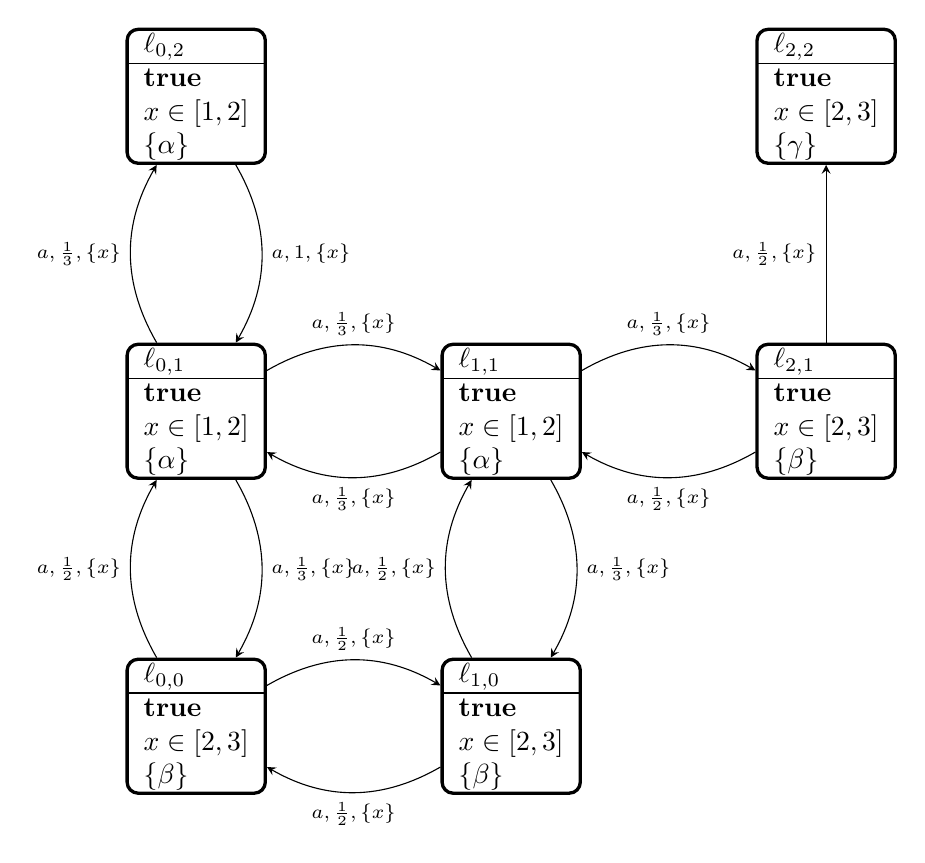
\begin{tikzpicture}[x=2cm, y=2cm]

\node[location] (q00)         at (0,0)
{
\begin{tabular}{l}
$\loc_{0,0}$\\
\hline
$\true$ \\
$x\in [2,3]$ \\
$\{\beta\}$
\end{tabular}
};

\node[location] (q01)         at (0,2)
{
\begin{tabular}{l}
$\loc_{0,1}$\\
\hline
$\true$ \\
$x\in [1,2]$ \\
$\{\alpha\}$
\end{tabular}
};

\node[location] (q02)         at (0,4)
{
\begin{tabular}{l}
$\loc_{0,2}$\\
\hline
$\true$ \\
$x\in [1,2]$ \\
$\{\alpha\}$
\end{tabular}
};

\node[location] (q10)         at (2,0)
{
\begin{tabular}{l}
$\loc_{1,0}$\\
\hline
$\true$ \\
$x\in [2,3]$ \\
$\{\beta\}$
\end{tabular}
};



\node[location] (q11)         at (2,2)
{
\begin{tabular}{l}
$\loc_{1,1}$\\
\hline
$\true$ \\
$x\in [1,2]$ \\
$\{\alpha\}$
\end{tabular}
};

\node[location] (q21)         at (4,2)
{
\begin{tabular}{l}
$\loc_{2,1}$\\
\hline
$\true$ \\
$x\in [2,3]$ \\
$\{\beta\}$
\end{tabular}
};

\node[location] (q22)         at (4,4)
{
\begin{tabular}{l}
$\loc_{2,2}$\\
\hline
$\true$ \\
$x\in [2,3]$ \\
$\{\gamma\}$
\end{tabular}
};

\draw[tran, bend left] (q00)       to node[auto, font=\scriptsize] {$a, \frac{1}{2}, \{x\}$}      (q01);
\draw[tran, bend left] (q00)       to node[auto, font=\scriptsize] {$a, \frac{1}{2}, \{x\}$}      (q10);
\draw[tran, bend left] (q01)       to node[auto, font=\scriptsize] {$a, \frac{1}{3}, \{x\}$}      (q11);
\draw[tran, bend left] (q01)       to node[auto, font=\scriptsize] {$a, \frac{1}{3}, \{x\}$}      (q00);
\draw[tran, bend left] (q01)       to node[auto, font=\scriptsize] {$a, \frac{1}{3}, \{x\}$}      (q02);
\draw[tran, bend left] (q02)       to node[auto, font=\scriptsize] {$a, 1, \{x\}$}      (q01);
\draw[tran, bend left] (q10)       to node[auto, font=\scriptsize] {$a, \frac{1}{2}, \{x\}$}      (q00);
\draw[tran, bend left] (q10)       to node[auto, font=\scriptsize] {$a, \frac{1}{2}, \{x\}$}      (q11);
\draw[tran, bend left] (q11)       to node[auto, font=\scriptsize] {$a, \frac{1}{3}, \{x\}$}      (q01);
\draw[tran, bend left] (q11)       to node[auto, font=\scriptsize] {$a, \frac{1}{3}, \{x\}$}      (q10);
\draw[tran, bend left] (q11)       to node[auto, font=\scriptsize] {$a, \frac{1}{3}, \{x\}$}      (q21);
\draw[tran, bend left] (q21)       to node[auto, font=\scriptsize] {$a, \frac{1}{2}, \{x\}$}      (q11);
\draw[tran] (q21)       to node[auto, font=\scriptsize] {$a, \frac{1}{2}, \{x\}$}      (q22);

\end{tikzpicture}
\caption{The PTA for Example~\ref{ex:robotnavigation}}
\label{fig:ptarobotnavigation}
\end{figure}

\begin{figure}
\centering
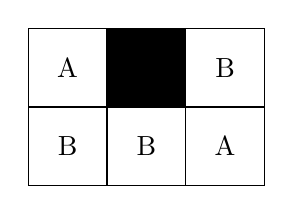
\begin{tikzpicture}[x = 1cm]
\begin{scope}
    \draw (0, 1) grid (3, 3);

    \setcounter{row}{1}
    \setrow{A}{ }{B}
    \setrow{B}{B}{A}
%    \node[anchor=center] at (1.5, -0.5) {Robot Navigation};
\end{scope}

\fill[black] (1,2) rectangle (2,3);

\end{tikzpicture}
\caption{A Robot-Navigation Example}
\label{fig:robotnavigation}
\end{figure}


%% A Previous Table

\begin{table}
\centering
\caption{Experimental Results for Task-Completion and Robot-Navigation}
\label{tab:er}
\begin{tabular}{|c|c|c|c|c|c|c|c|c|c|}
\hline
\multicolumn{5}{|c|}{Task-Completion} & \multicolumn{5}{|c|}{Robot-Navigation}\\
\hline
$N$ & Size & Time & max & min & $N$ & Size & Time & max & min \\
\hline
5& & & & & 4& & & &\\
\hline
7& & & & & 5& & & &\\
\hline
9& & & & & 6& & & &\\
\hline
11& & & & & 7& & & &\\
\hline
13& & & & & 8& & & &\\
\hline
15& & & & & 9& & & &\\
\hline
15& & & & & 10& & & &\\
\hline
\end{tabular}
\end{table}

%% Another Previous Table

\begin{table}
\caption{Experimental Results for Robot-Navigation}
\label{tab:robotnavigation}
\centering
\begin{tabular}{|c|c|c|c|c|}
\hline
$N$ & Size & Time & min & max \\
\hline
4& 1971 & 14s & 0.2166 & 0.3799 \\
\hline
5& 3390 & 54s & 0.1672 & 0.3146 \\
\hline
6& 7368 & 339s & 0.0724 & 0.1753 \\
\hline
7& 9873 & 1007s & 0.0473 & 0.1233 \\
\hline
8& 18131 & 2991s & 0.0200 & 0.0607 \\
\hline
9& 21564 & 6080s & 0.0092 &0.0371 \\
\hline
10& 36210 & 13383s & 0.0076 &0.0329 \\
\hline
\end{tabular}
\end{table}

